\documentclass[12pt]{report}
\usepackage{outline} 
\usepackage{pmgraph} 
\usepackage[normalem]{ulem}
\usepackage{graphicx} 
\usepackage{verbatim}
\usepackage{amsmath}
\usepackage{subfigure}
\usepackage{indentfirst}
\usepackage{float}

\title{

\includegraphics[width=1.7in]{RI_Logo.png} \\
\vspace*{1in}
\textbf{Visual Learning \& Recognition Assignment \uppercase\expandafter{\romannumeral1}}}
\author{\textbf{Jiahong Ouyang} \\
	ID: jiahongo@andrew.cmu.edu\\
		\vspace*{0.5in} \\
		MRSD Program, Robotic Institute\\
        \textbf{Carnegie Mellon University}\\
        Pittsburgh, PA
       } \date{\today}
       
%--------------------Make usable space all of page
\setlength{\oddsidemargin}{0in} 
\setlength{\evensidemargin}{0in}
\setlength{\topmargin}{0in}     
\setlength{\headsep}{-.25in}
\setlength{\textwidth}{6.5in}   
\setlength{\textheight}{8.5in}
%--------------------Indention
\setlength{\parindent}{1cm}


\begin{document}
%--------------------Title Page
\maketitle
%--------------------Begin Outline
\begin{outline}

%--------------------------task1
\item \textbf{Task 0:  MNIST 10-digit classification in TensorFlow}\\
\textbf{Q 0.1: What test accuracy does your model get?}\\
After training for 20,000 iterations, the test accuracy is 96.97\%.\\

\textbf{Q 0.2: What happens if you train for more iterations (30000)?}\\
After training for 20,000 iterations, the test accuracy is still going up. The test accuracy is 97.69\% after 30,000 iterations. But training too much, the test accuracy will start to decrease because of the overfitting.\\

\textbf{Q 0.3: Make the training loss and validation accuracy curve. Show for at least 100 points between 0 to 20000 iterations.}

\begin{figure*}[!h]
  \centering
  \subfigure[]{
    \label{fig:subfig:a}
    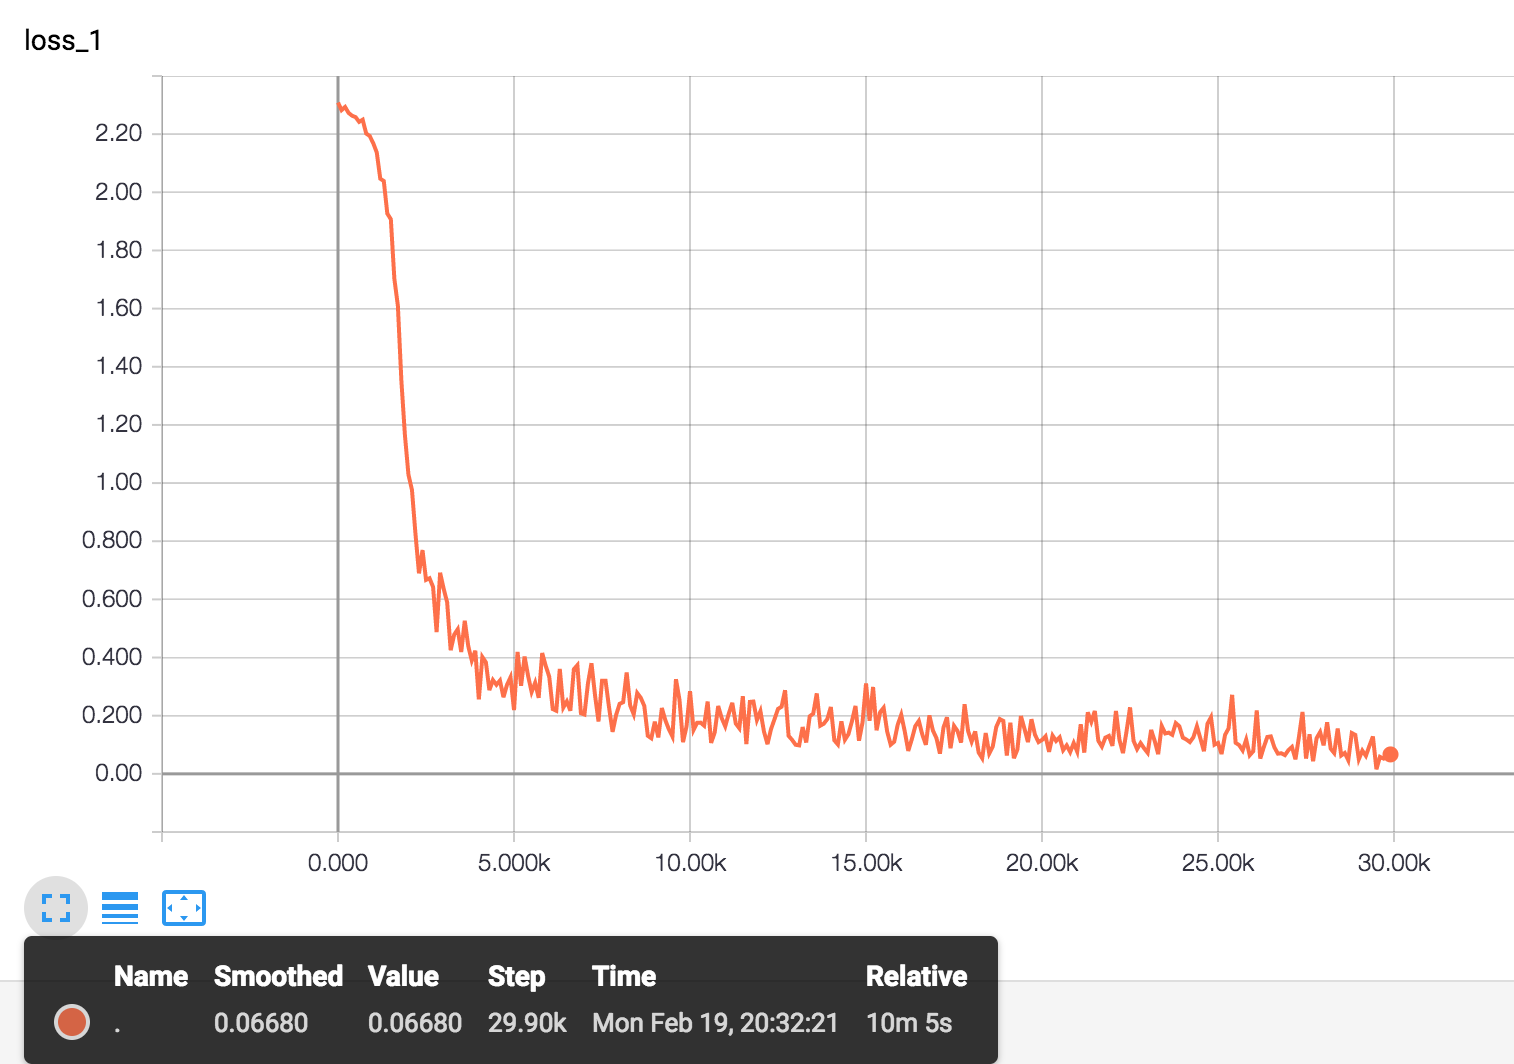
\includegraphics[width=3in]{task0_loss_30k.png}}
  %\hspace{0.01in}
  \subfigure[]{
    \label{fig:subfig:b} 
    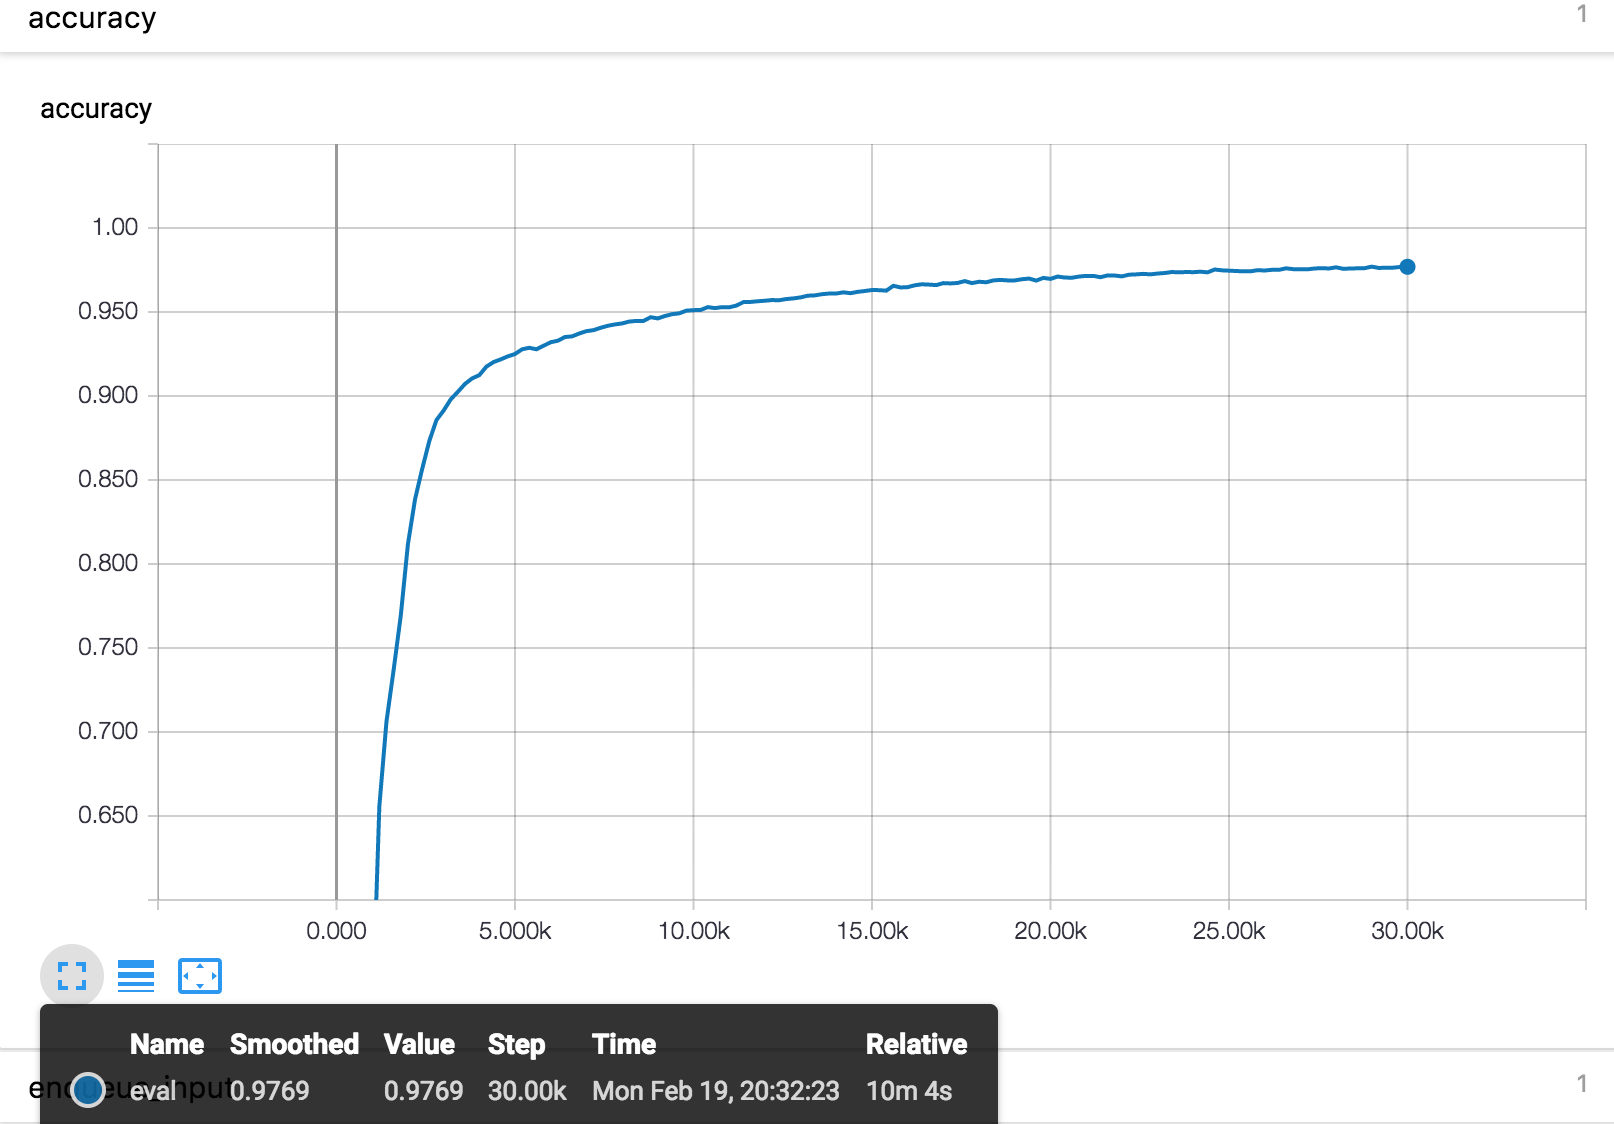
\includegraphics[width=3in]{task0_acc_30k.png}}
  \caption{Task0: Training loss and validation accuracy curve}
  %\label{fig:subfig} 
\label{fig:short}
\end{figure*}

\item \textbf{Task 1: 2-layer network for PASCAL multi-label classification}\\

\textbf{Q 1.3: Same as before, show the training and accuracy (mAP) curves. Train for only 1000 iterations.}\\
As the structure of the 2-layer network is too easy, the final result is not good. It only achieved 18\% mAP.\\

\begin{figure*}[!h]
  \centering
  \subfigure[]{
    \label{fig:subfig:a}
    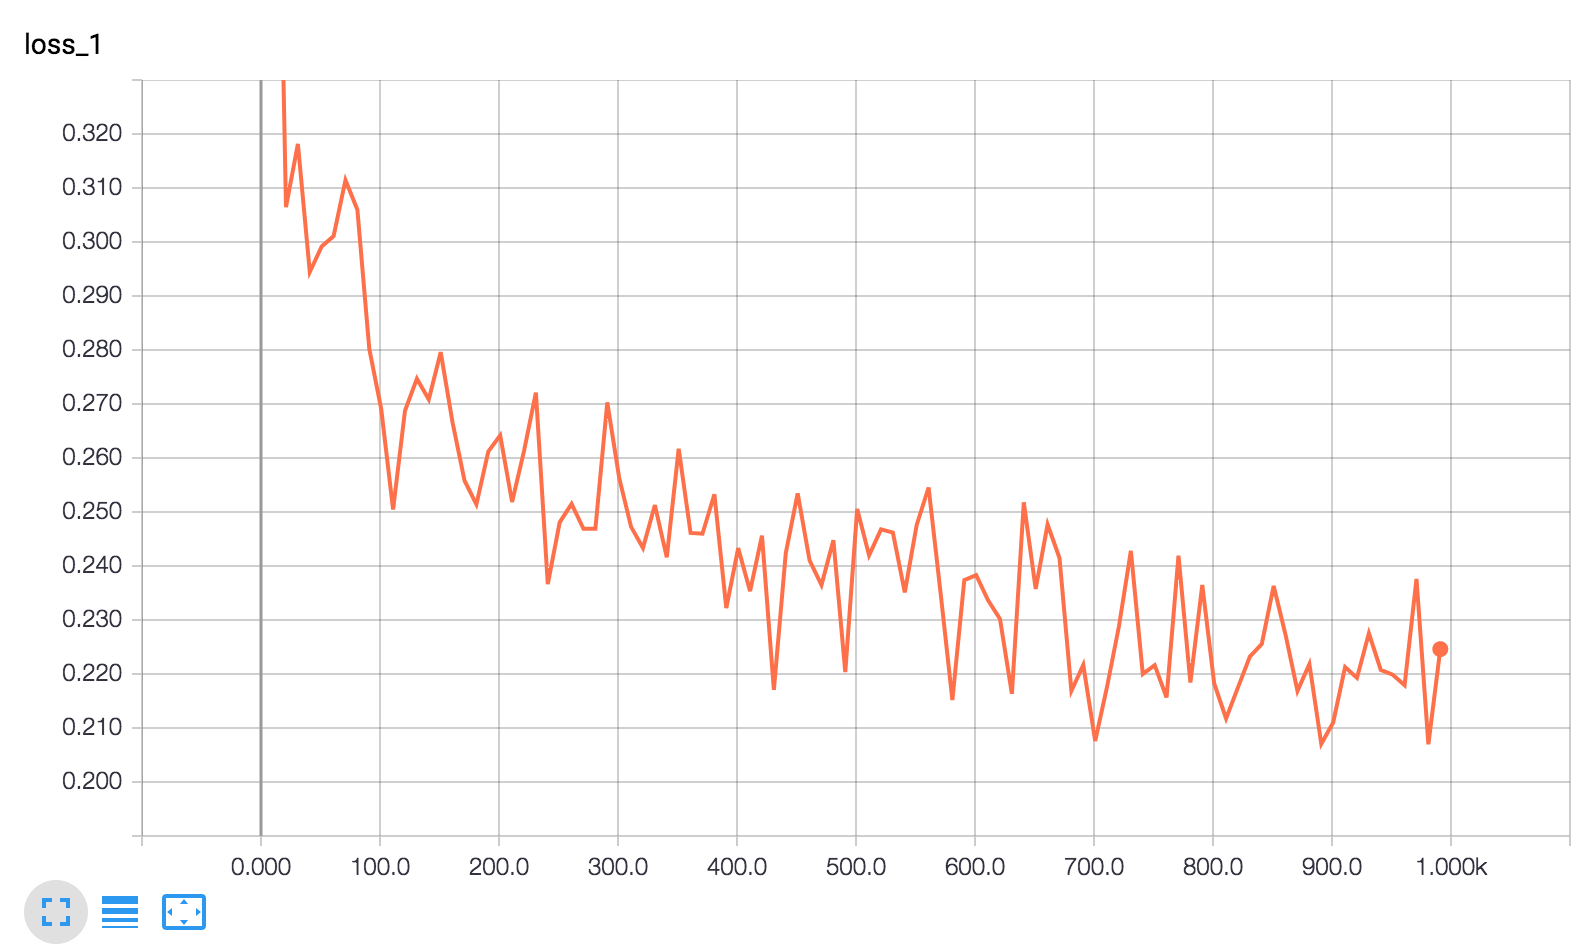
\includegraphics[width=3in]{task1_loss.png}}
  %\hspace{0.01in}
  \subfigure[]{
    \label{fig:subfig:b} 
    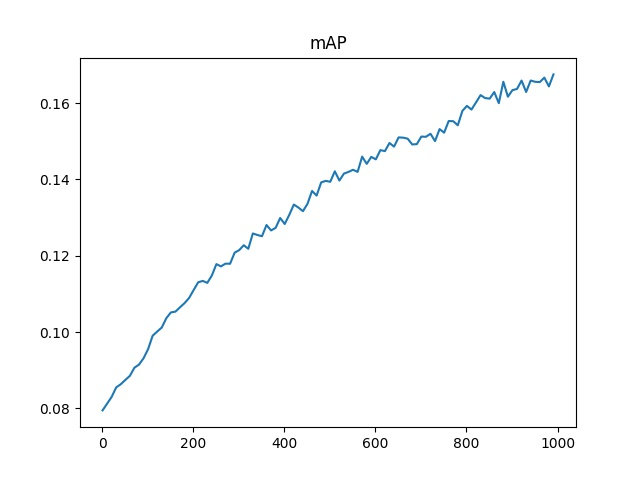
\includegraphics[width=3in]{task1_mAP_plot.jpg}}
  \caption{Task1: Training loss and mAP curve for 2-layer network on PASCAL}
  %\label{fig:subfig} 
\label{fig:short}
\end{figure*}


\item \textbf{Task 2: Lets go deeper! AlexNet for PASCAL classification}\\

For AlexNet, I tried different data processing methods to train the model. First, I directly feed images to the network, which means the intensity of image is integer in [0, 255] with Gaussian initailzer for conv2d and dense's weights and zero initializer for bias. I got the mAP of 33.47\%. Second, I subtracted the mean from the raw image and also transfer it into [-1, 1] and used the same initializer and parameters. Theoratically, after doing the normalization, the accuracy should be higher, but actually the fact is the opposite. The mAP of second way is only 9.45\% Maybe transforming it into [0,1] will have better results. \\
For data augmentation, I only did the random cropping and random left-right flipping. I also tried randomly changing image's contrast or adding gaussian noise, but maybe because it changed the image too much, thus didn't get good results.\\

\textbf{Q 2.3: Implement the data augmentation and generate the loss and mAP curves as before.}\\
The data augmentation method is described above.\\ 

\begin{figure*}[!h]
  \centering
  \subfigure[]{
    \label{fig:subfig:a}
    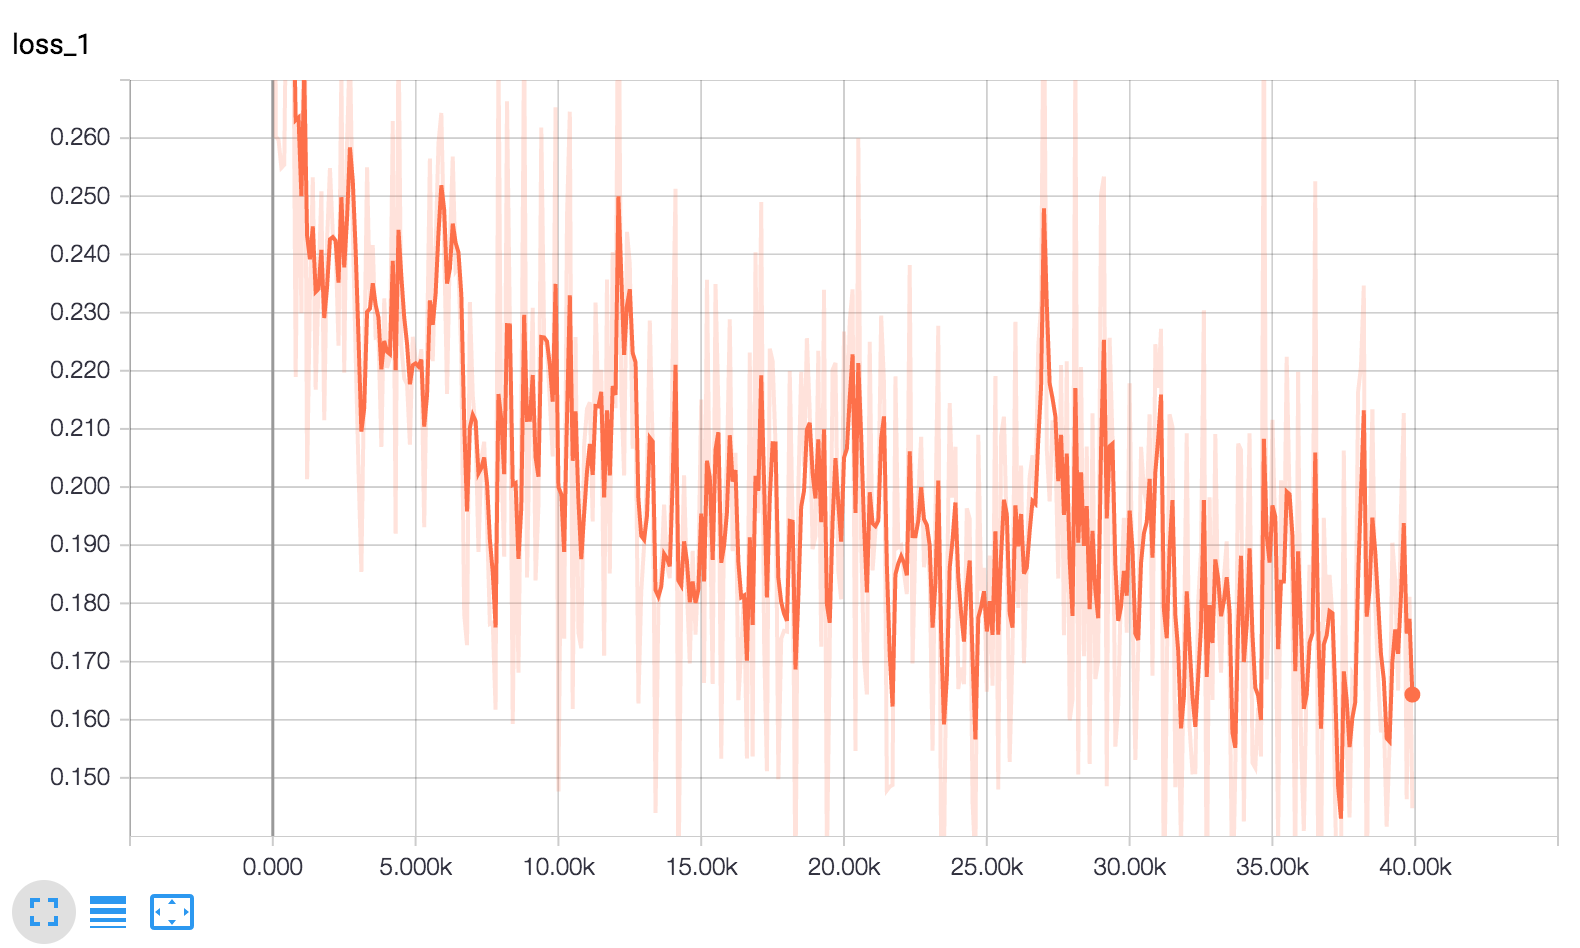
\includegraphics[width=3in]{task2_loss.png}}
  %\hspace{0.01in}
  \subfigure[]{
    \label{fig:subfig:b} 
    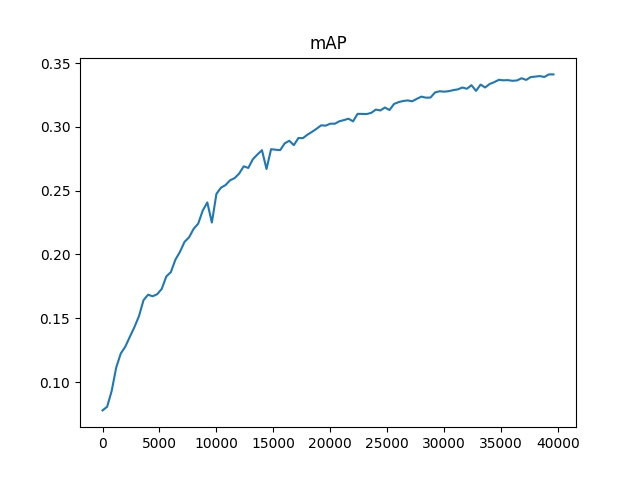
\includegraphics[width=3in]{task2_mAP_plot.jpg}}
  \caption{Task3: Training loss and mAP curve for AlexNet on PASCAL}
  %\label{fig:subfig} 
\label{fig:short}
\end{figure*}

\item \textbf{Task 3: Even deeper! VGG-16 for PASCAL classification}\\

For VGG16, I tried different parameter configurations. I tried with and without normalization, with and without initializer. I only got is 8.15\% mAP after 30k iterations with normalization and without initialzer (method 1). Then I found out that when training VGG16, people usually only subtract the mean from the images without transforming to [0, 1] or [-1,1]. Meanwhile, to better train the model, I added random brightness adjustment, random contrast adjustment and random Gaussian noise for data augmentation (method 2). When I used this method, I achieved 30.2\% mAP after 20k iterations. \\

One thing that I can't understand is that why the normalization will benefit the VGG16 while hurt the AlexNet. If that's the case, is there a way that we can follow to train different models?\\

\textbf{Q 3.1: Modify the network architecture from Task 2 to implement the VGG-16 architecture (refer to the original paper). Use the same hyperparameter settings from Task 2, and try to train the model. Add the train/test loss/accuracy curves into the report.}\\

The final mAP I achieved is 30.2\%.

\begin{figure*}[!h]
  \centering
  \subfigure[]{
    \label{fig:subfig:a}
    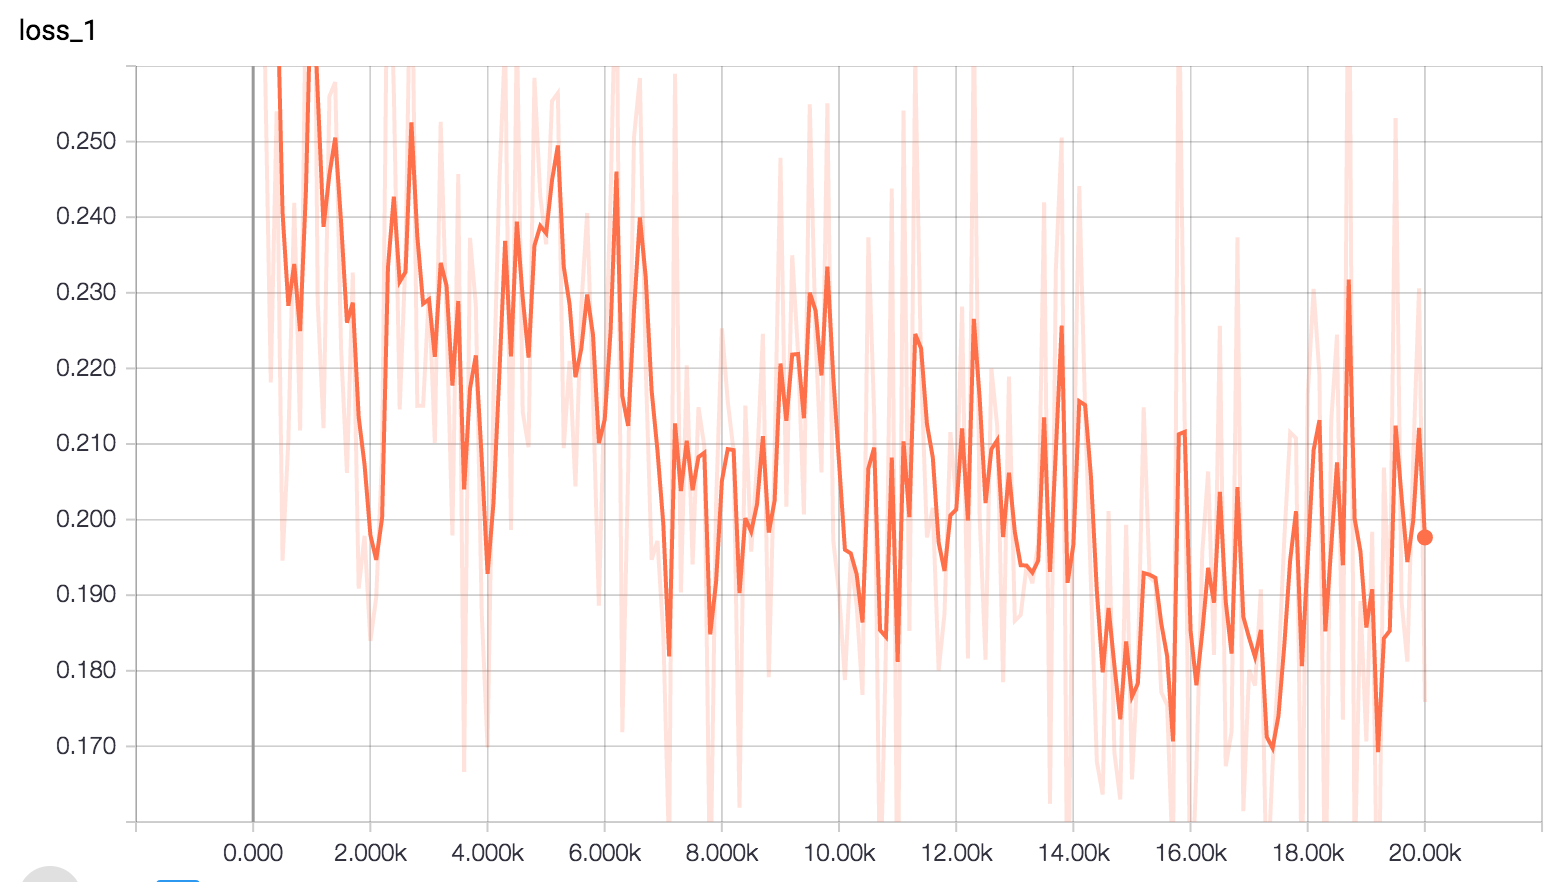
\includegraphics[width=3in]{task3_loss_2.png}}
  %\hspace{0.01in}
  \subfigure[]{
    \label{fig:subfig:b} 
    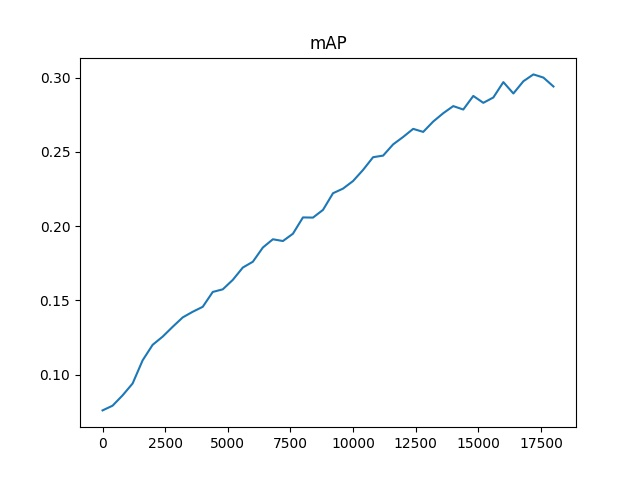
\includegraphics[width=3in]{task3_vgg16_mAP_plot.jpg}}
  \caption{Task3: Training loss and mAP curve for VGG16 on PASCAL(method 2)}
  %\label{fig:subfig} 
\label{fig:short}
\end{figure*}

\textbf{Q 3.2: The task in this section is to log the following entities: a) Training loss, b) Learning rate, c) Histograms of gradients, d) Training images and e) Network graph into tensorboard. Add screenshots from your tensorboard into the report.}\\

\begin{figure*}[!h]
  \centering
  \subfigure[]{
    \label{fig:subfig:a}
    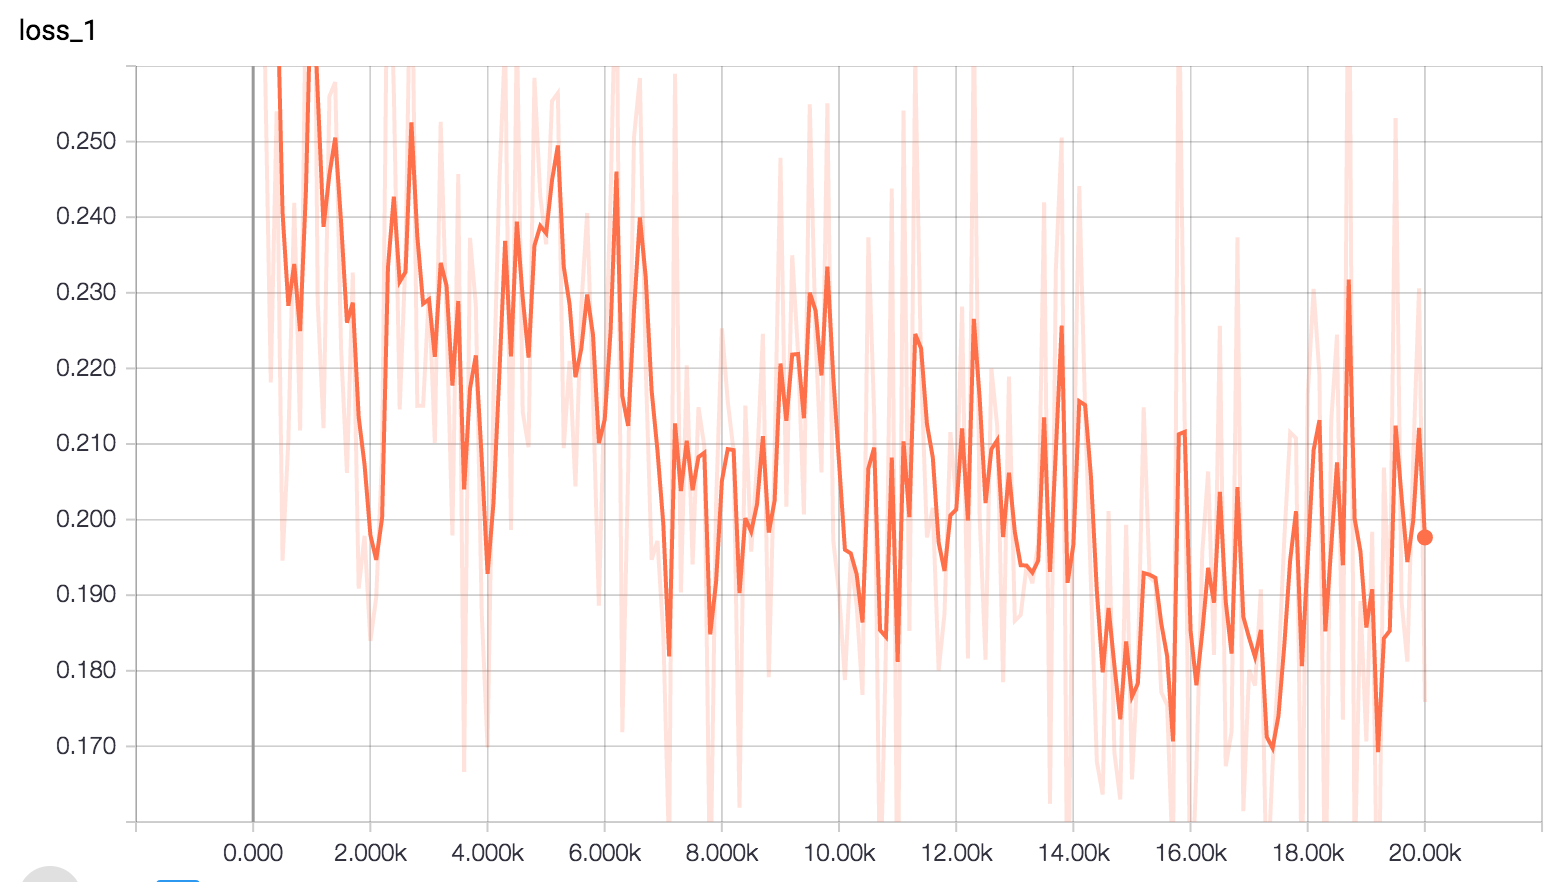
\includegraphics[width=2.8in]{task3_loss_2.png}}
  %\hspace{0.01in}
  \subfigure[]{
    \label{fig:subfig:b} 
    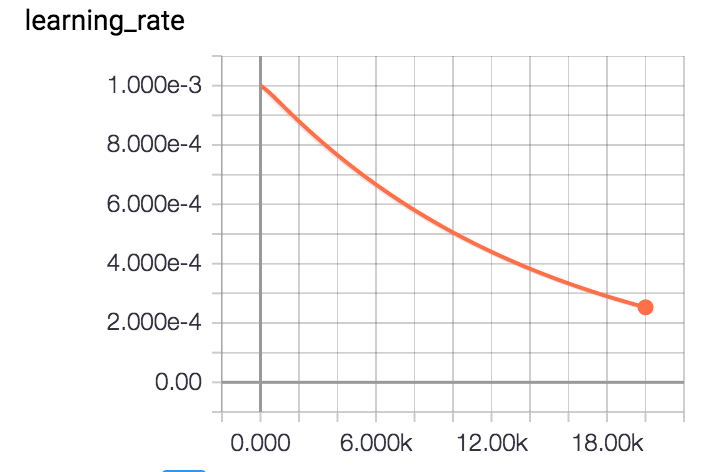
\includegraphics[width=2.8in]{task3_lr_2.png}}
   \subfigure[]{
    \label{fig:subfig:c}
    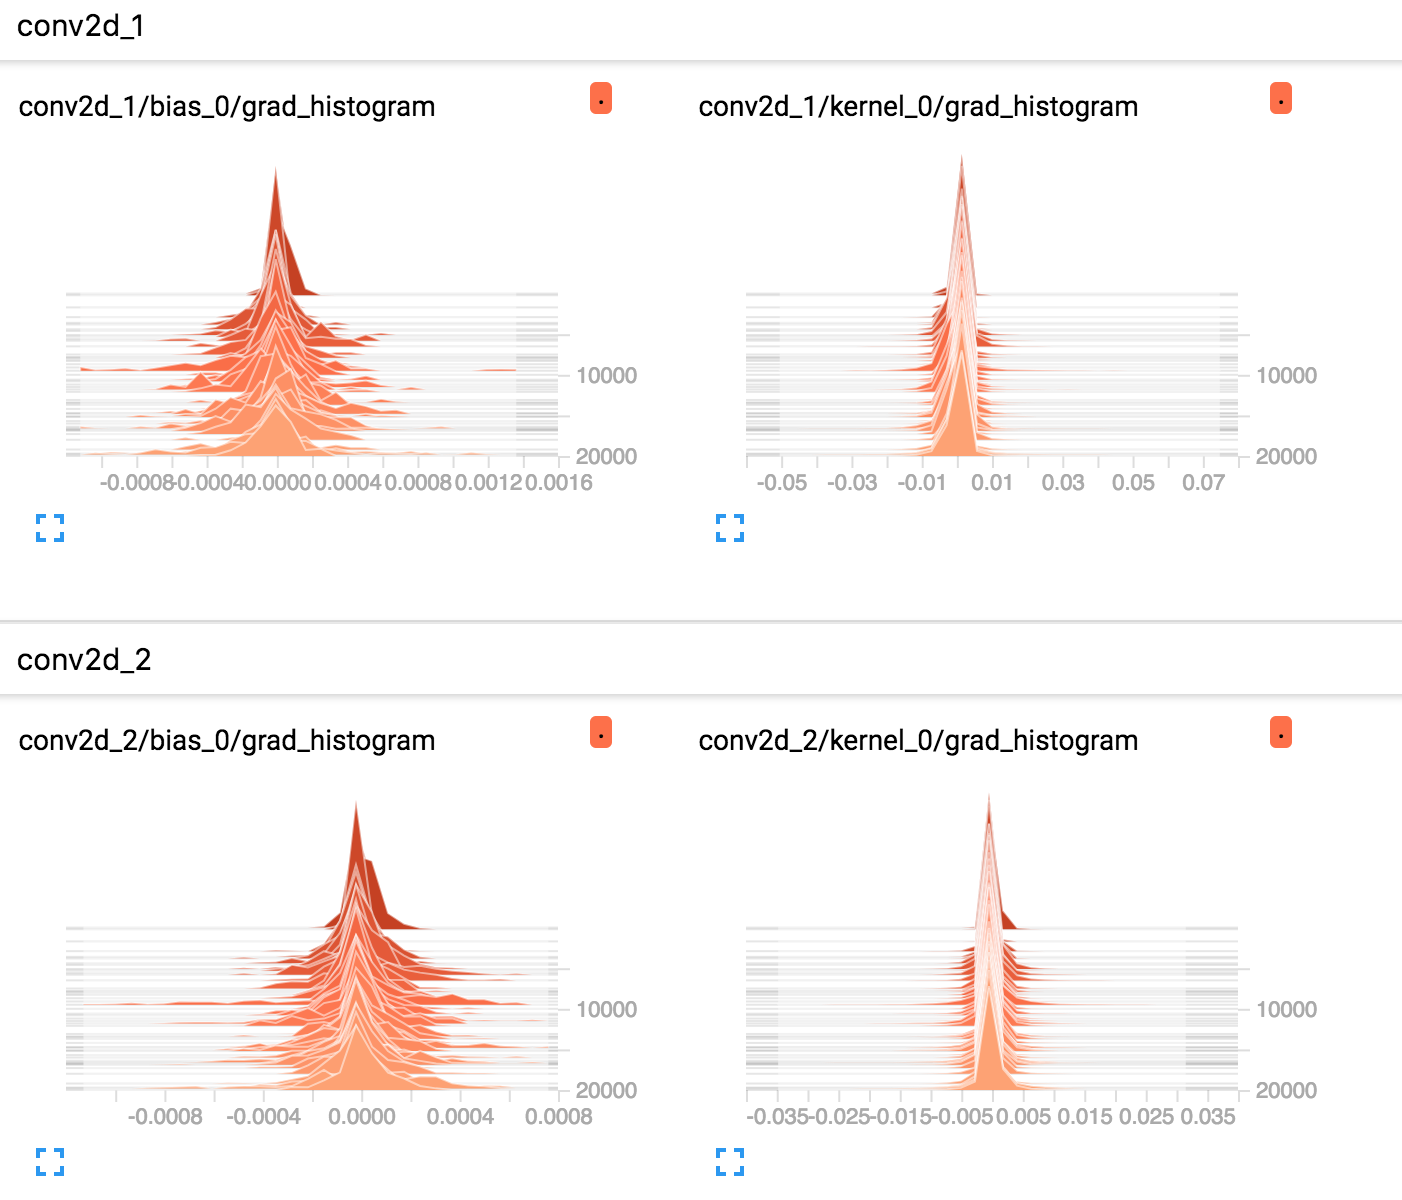
\includegraphics[width=2.8in]{task3_histogram_2.png}}
  %\hspace{0.01in}
  \subfigure[]{
    \label{fig:subfig:d} 
    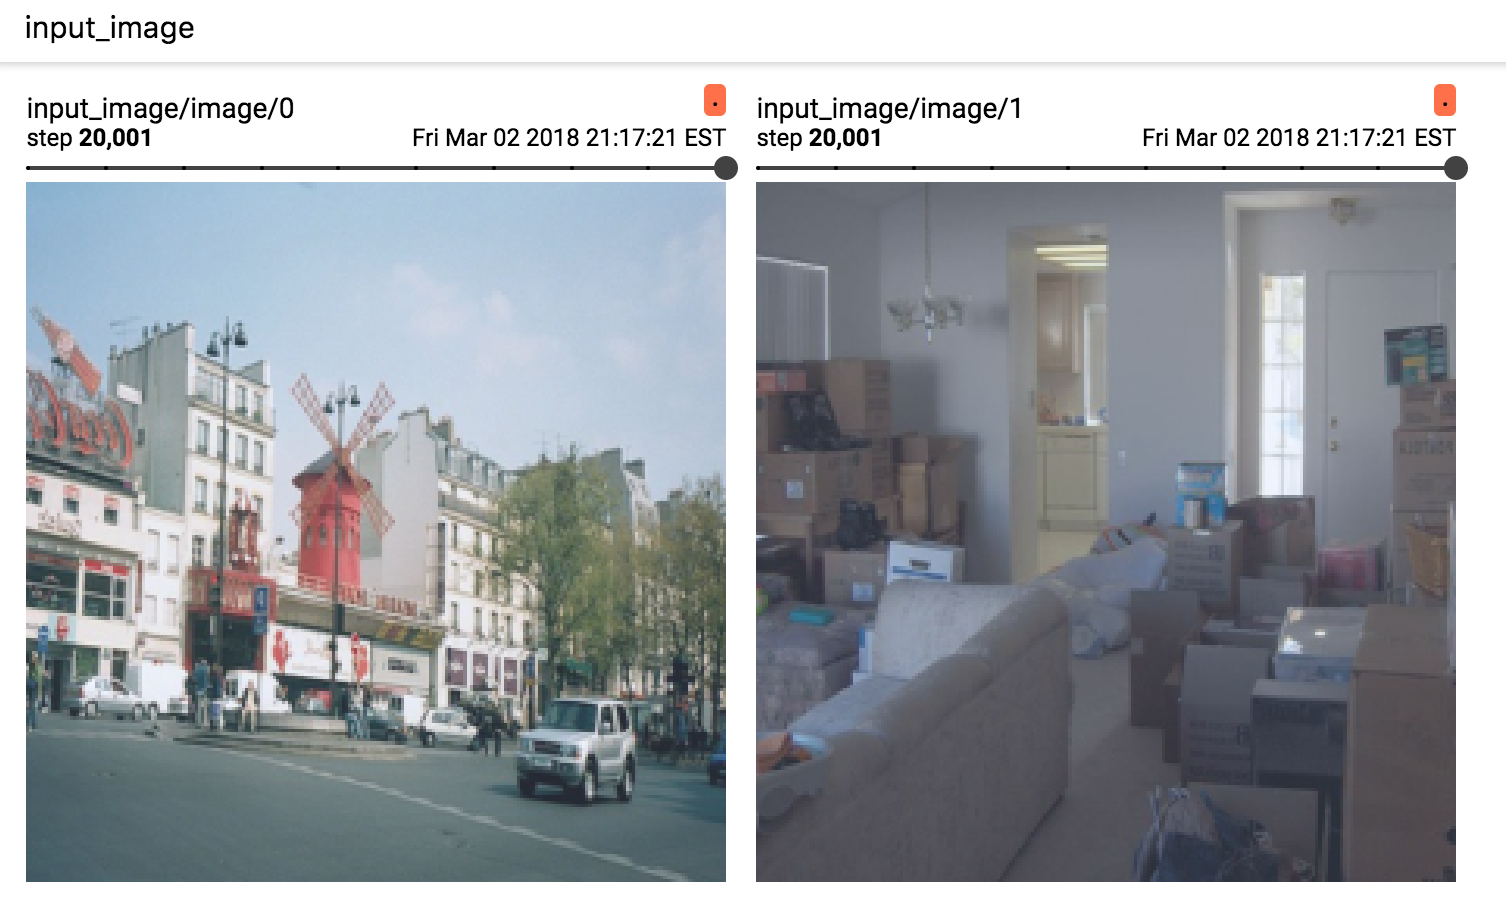
\includegraphics[width=2.8in]{task3_image_2.png}}
    \subfigure[]{
    \label{fig:subfig:e} 
    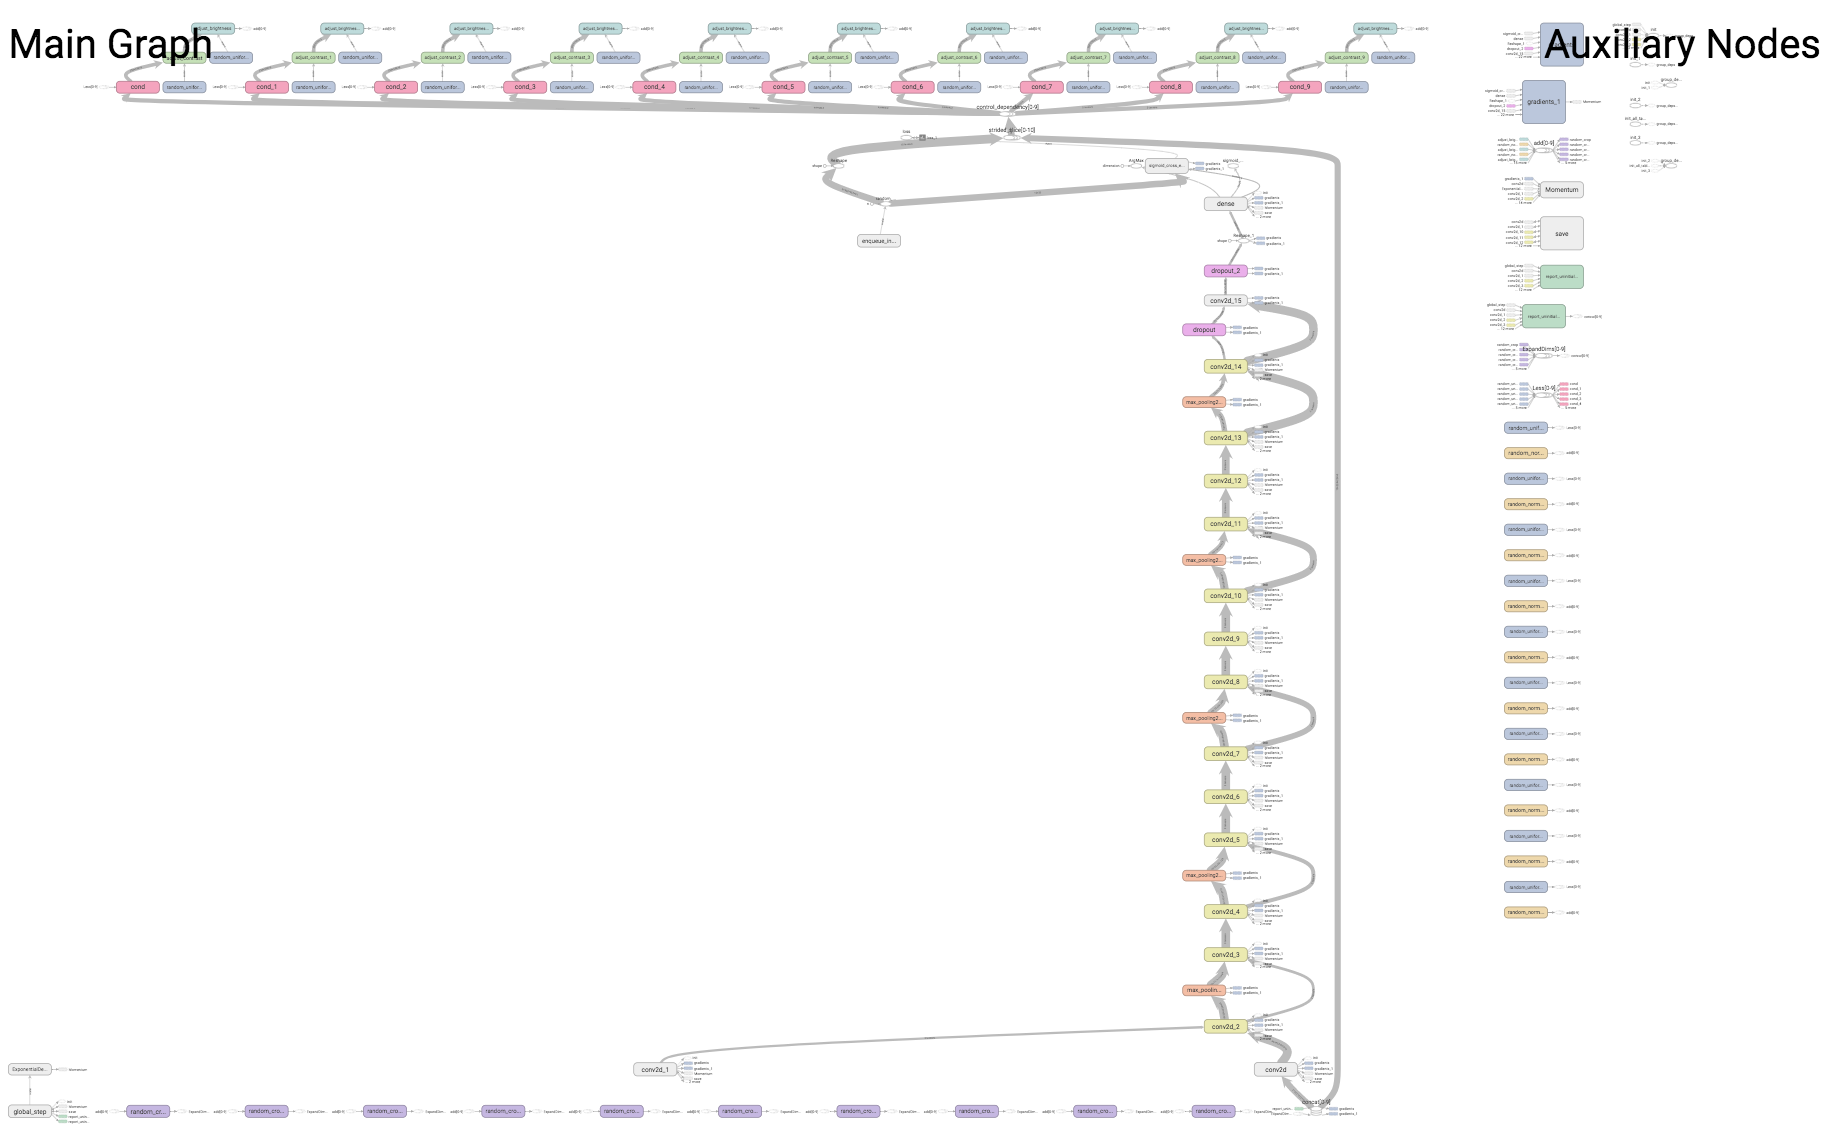
\includegraphics[width=5.5in]{task3_graph_2.png}}
  \caption{Task3: Screenshots of Tensorboard for VGG16 on PASCAL (method 2)}
  %\label{fig:subfig} 
\label{fig:short}
\end{figure*}

\item \textbf{Task 4: Standing on the shoulder of the giants: fine-tuning from ImageNet}\\

For fine-tuning the network, I loaded the parameters except for the last dense layer. According to the homework instruction, we should keep 1/10th of the learning rate of task 3 and learning rate decay step should be also 1/10th. But I found out that if the learning rate is too small, the training process is too slow, thus I need to train more than 4k iterations to get a relative satisfying results. So I kept the same learning rate and trained the model. \\

\textbf{Q 4.1: Load the pre-trained weights upto fc7 layer, and initialize fc8 weights and biases from scratch. Then train the network as before and report the training/validation curves and final performance on PASCAL test set.}\\

The results is shown in figure 6. The final mAP is around 83\%.\\

\begin{figure*}[!h]
  \centering
  \subfigure[]{
    \label{fig:subfig:a}
    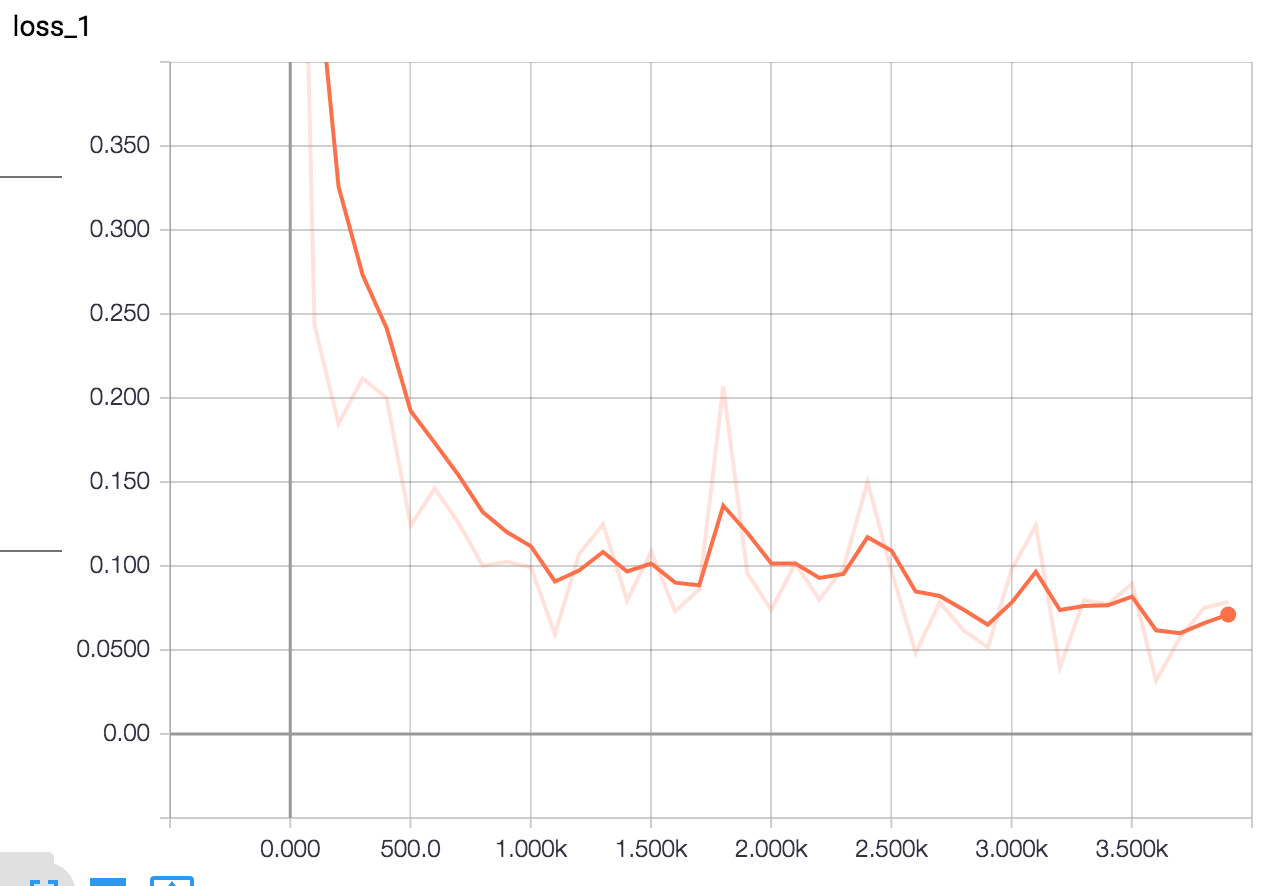
\includegraphics[width=3in]{task4_loss.png}}
  %\hspace{0.01in}
  \subfigure[]{
    \label{fig:subfig:b} 
    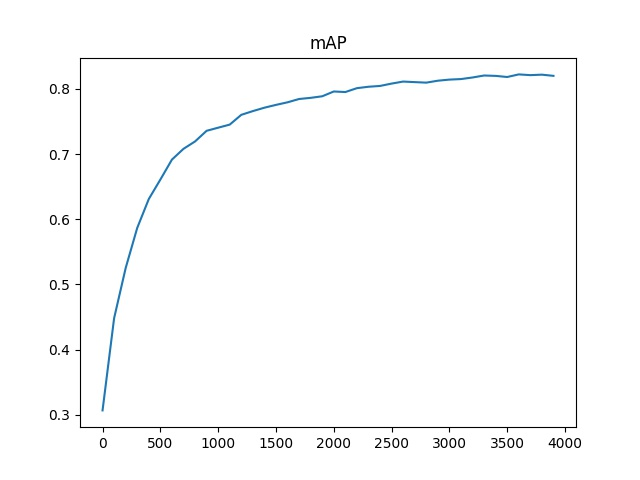
\includegraphics[width=3in]{task4_mAP_plot.jpg}}
  \caption{Task4: Training loss and mAP curve for VGG16 with pretrained model on PASCAL}
  %\label{fig:subfig} 
\label{fig:short}
\end{figure*}

\item \textbf{Task 5: Analysis}\\

\textbf{Conv-1 filters}\\

I extracted the filters of the first convolutional layer of AlexNet in task 2. As I used the The filters at iteration 2, 4k, 28k and 40k is shown below. As we can see, with the training process, the filters gradually have better representation ability, which can convey some low-level features just like Gabor filter.\\

\begin{figure*}[!h]
  \centering
  \subfigure[]{
    \label{fig:subfig:a}
    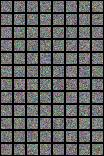
\includegraphics[width=1.5in]{task5_alexnet_conv1_filters_2.jpg}}
  %\hspace{0.01in}
  \subfigure[]{
    \label{fig:subfig:b} 
    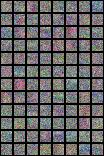
\includegraphics[width=1.5in]{task5_alexnet_conv1_filters_4000.jpg}}
   \subfigure[]{
    \label{fig:subfig:c}
    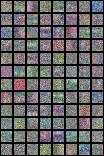
\includegraphics[width=1.5in]{task5_alexnet_conv1_filters_28000.jpg}}
  %\hspace{0.01in}
  \subfigure[]{
    \label{fig:subfig:d} 
    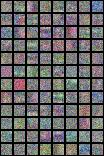
\includegraphics[width=1.5in]{task5_alexnet_conv1_filters_40000.jpg}}
  \caption{Task5: Conv-1 filters of AlexNet}
  %\label{fig:subfig} 
\label{fig:short}
\end{figure*}

\textbf{Nearest Neighbours}\\

I randomly picked 15 images from the test dataset and used features from pool5 and fc7 of AlextNet and VGG16 to found the 5 nearest neighbours in the test dataset respectively. Theoratically, the first nearest neighbour should be the test image itself and the other neighbours should be the images that contain the same object category or have similar features.

Comparing the pool5 and fc7, we can see that fc7 has better performance finding the nearest, which is very obvious in VGG16 that there are some ambigous images that match to many selected images. This convinces the assumption that higher layer can better convey the global and high-level features.

Comparing the AlexNet and VGG16, the latter results are much better than the AlexNet. For AlexNet, it works well on some images that have obvious features, like the train and the horse. But for some images that contain more than one object, like the one the ma with dog (6th) and life scene (5th, 7th) or have less features, like the computer (14th). For VGG16, almost all the matches are correct and for the one that is misclassified we can also get the clue of the reason. Sometimes, when the object is too small in the image, the feature is hard to extract or the two object categories are similar to each other, such as cow and sheep, cat and dog.\\

\begin{figure*}[!h]
  \centering
  \subfigure[]{
    \label{fig:subfig:a}
    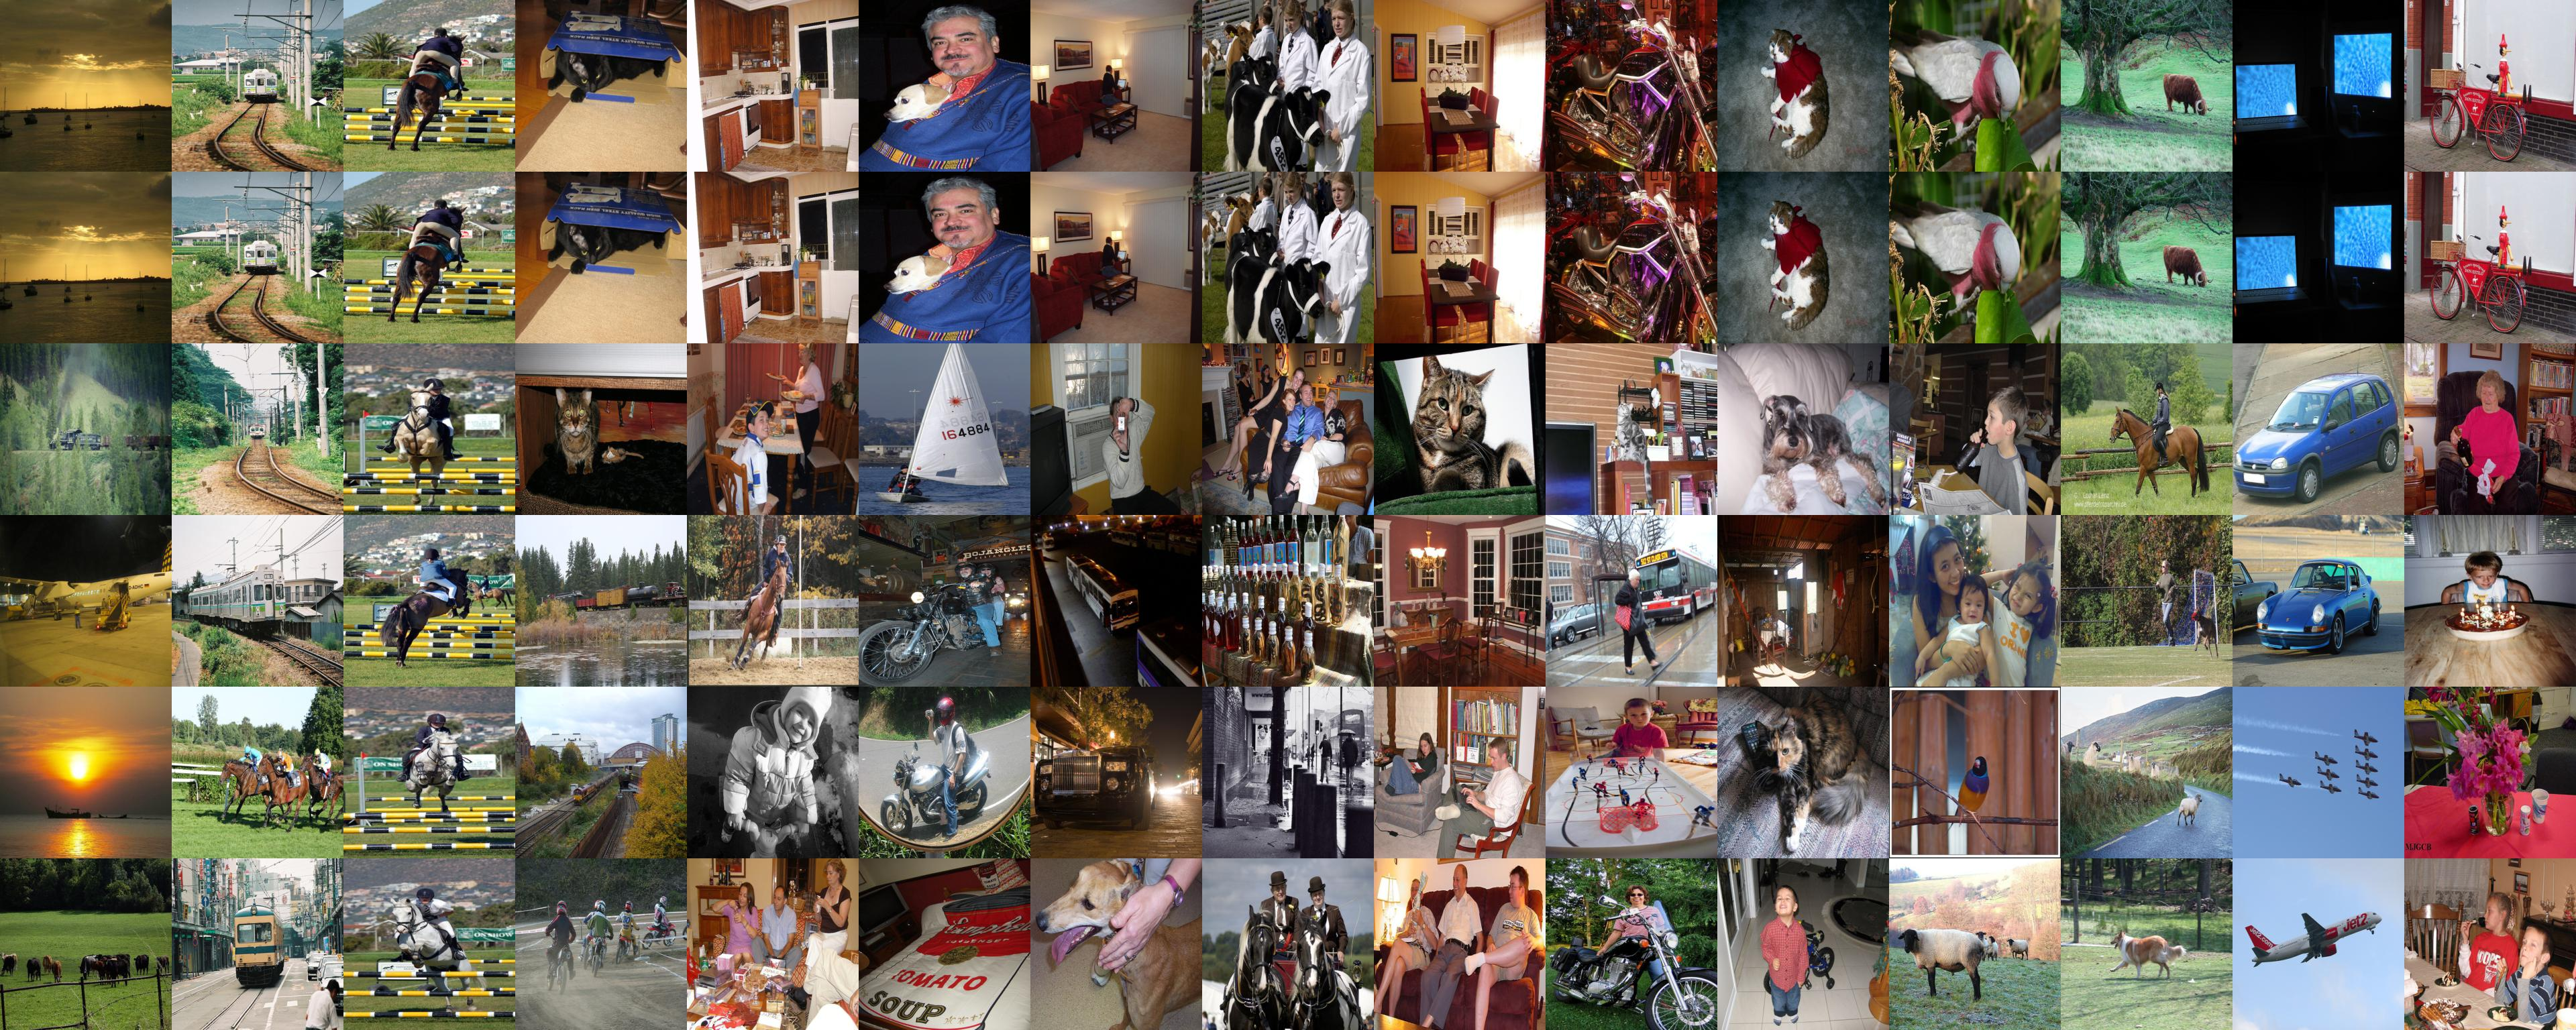
\includegraphics[width=7in]{task5_kNN_alexnet_pool5.jpg}}
  %\hspace{0.01in}
  \subfigure[]{
    \label{fig:subfig:b} 
    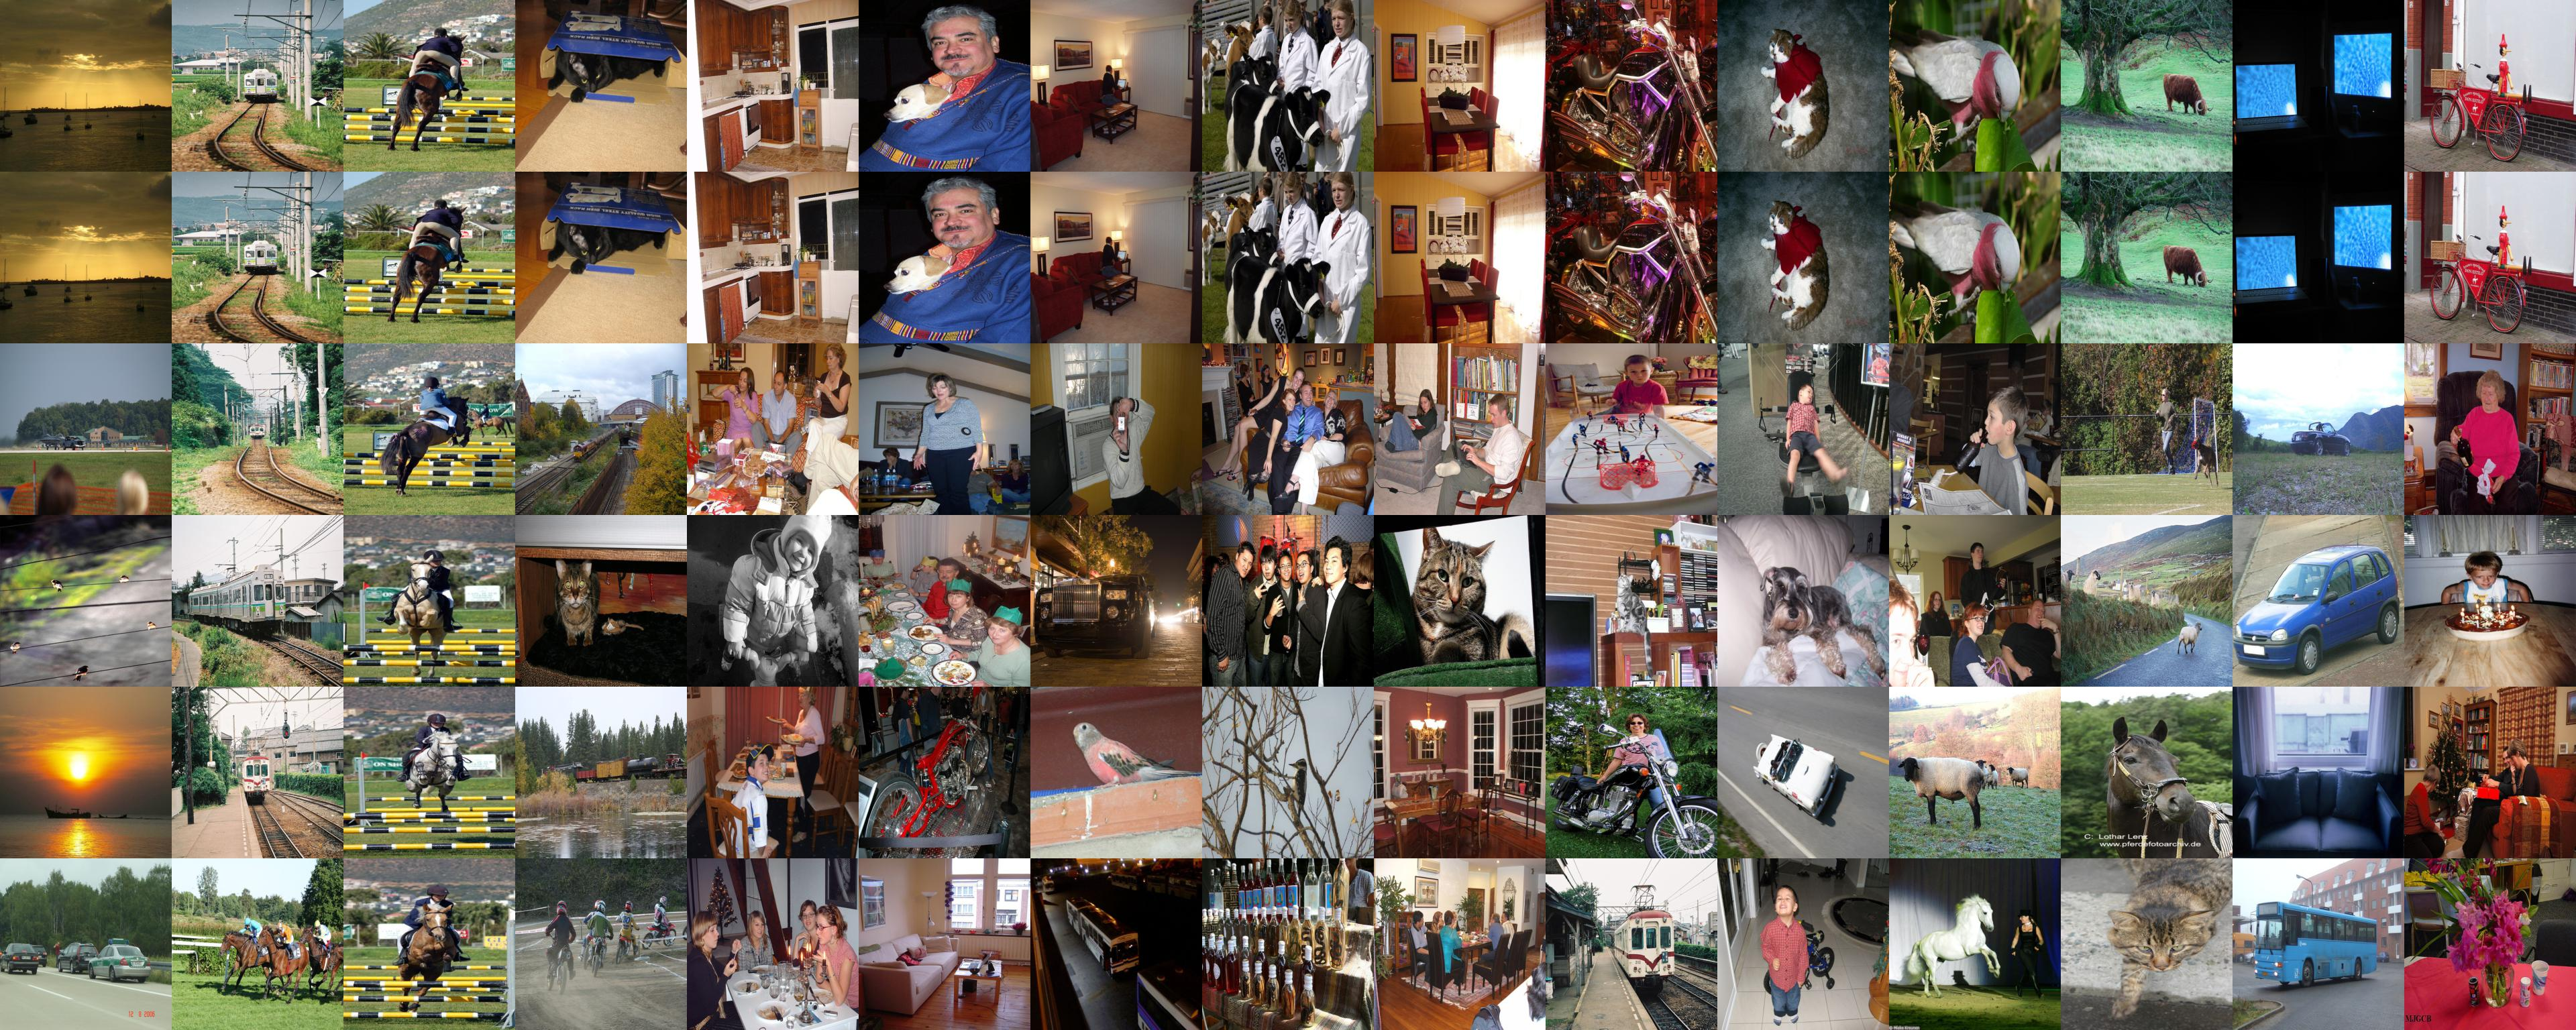
\includegraphics[width=7in]{task5_kNN_alexnet_fc7.jpg}}
  \caption{Task5: 5 Nearest Neighbours by pool5(a) and fc7(b) features of AlexNet. The first line is the test images and lines below are their neighbours.}
  %\label{fig:subfig} 
\label{fig:short}
\end{figure*}

\begin{figure*}[!h]
  \centering
  \subfigure[]{
    \label{fig:subfig:a}
    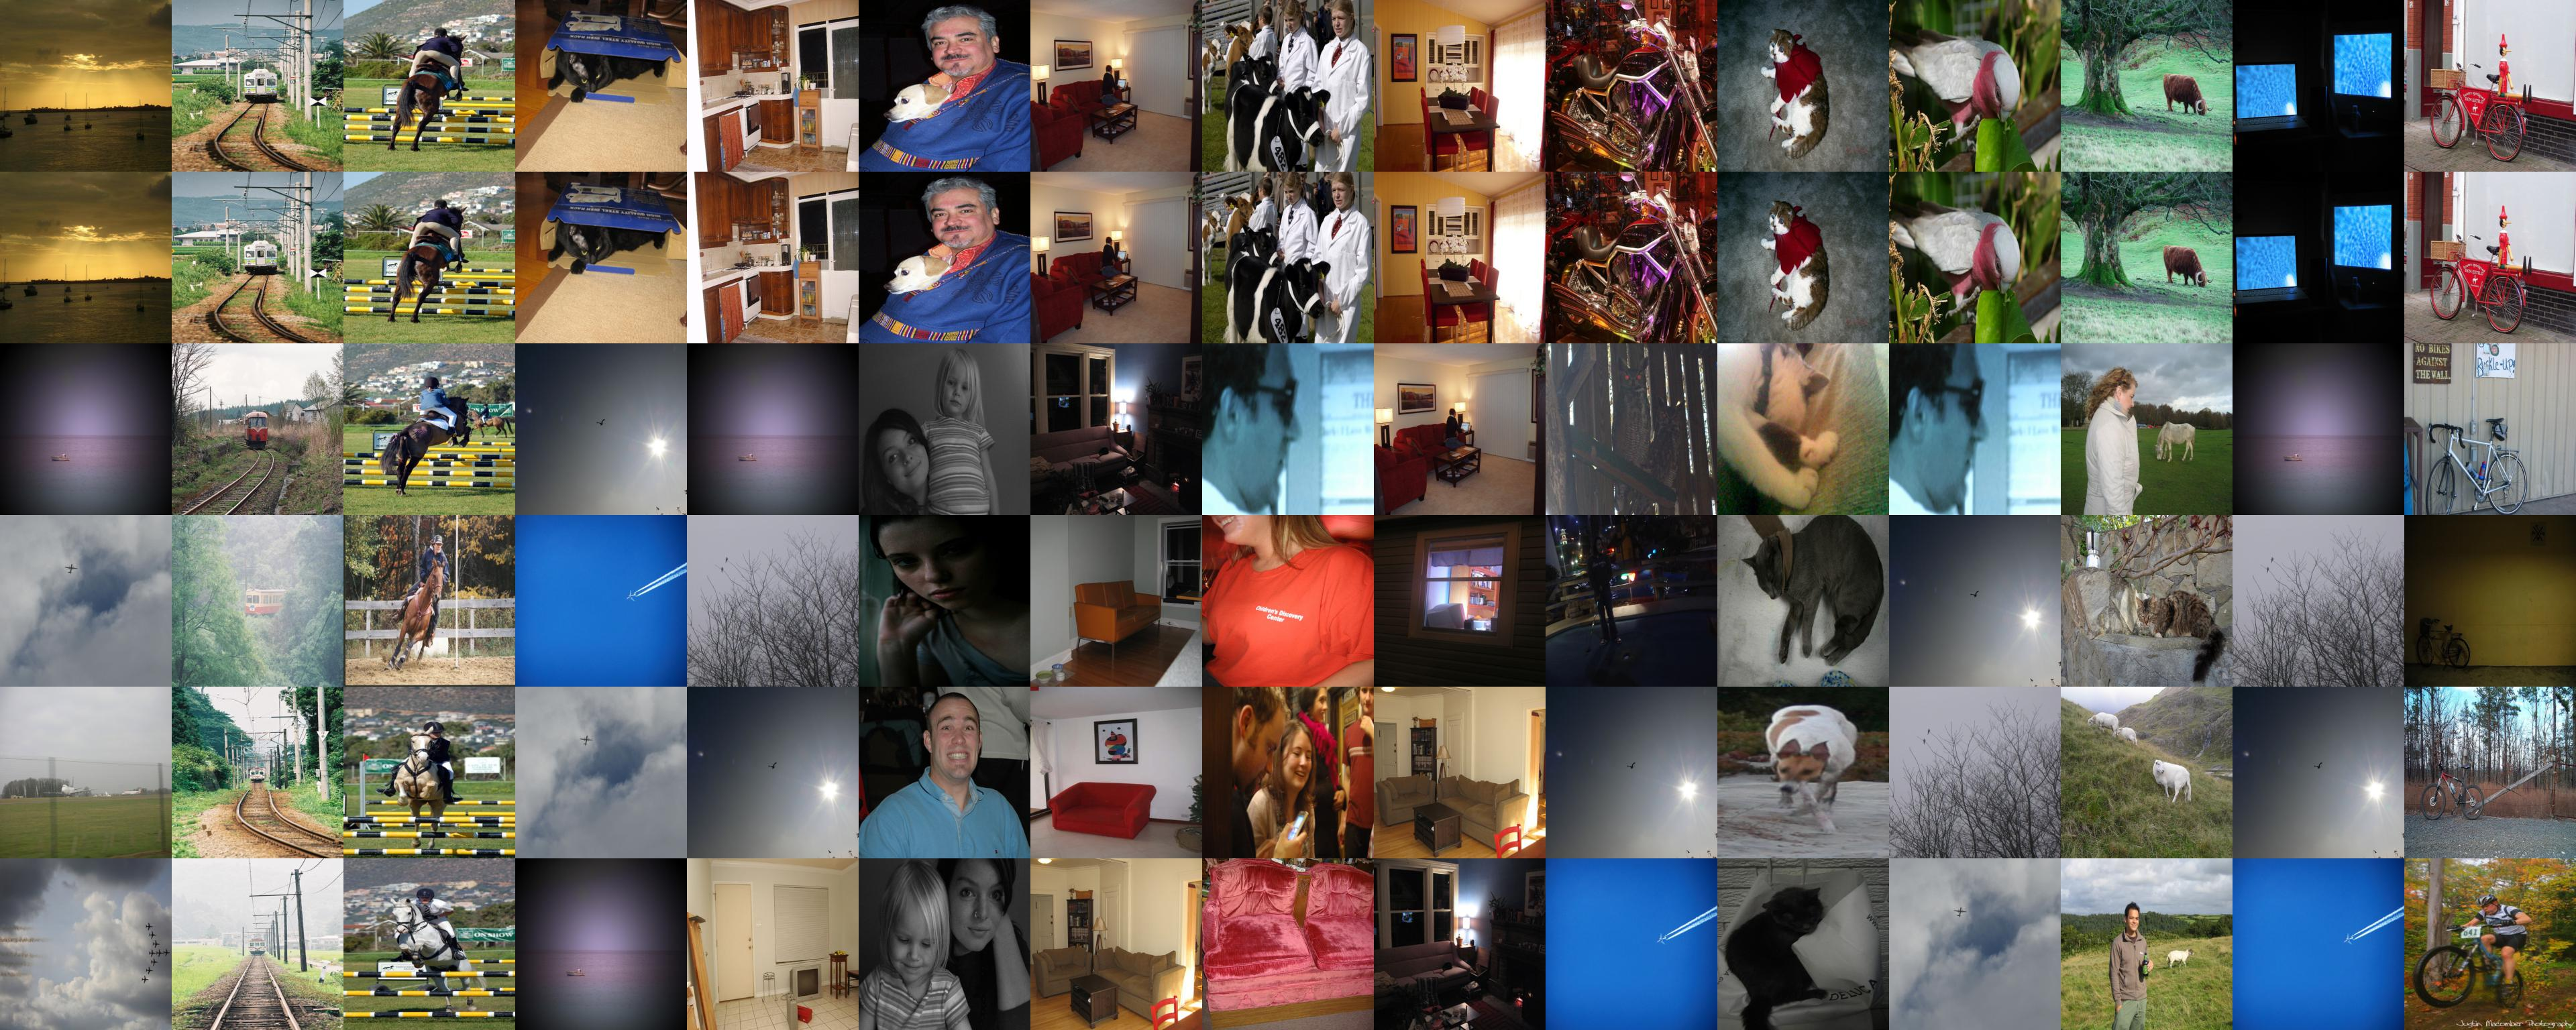
\includegraphics[width=7in]{task5_kNN_vgg16_pool5.jpg}}
  %\hspace{0.01in}
  \subfigure[]{
    \label{fig:subfig:b} 
    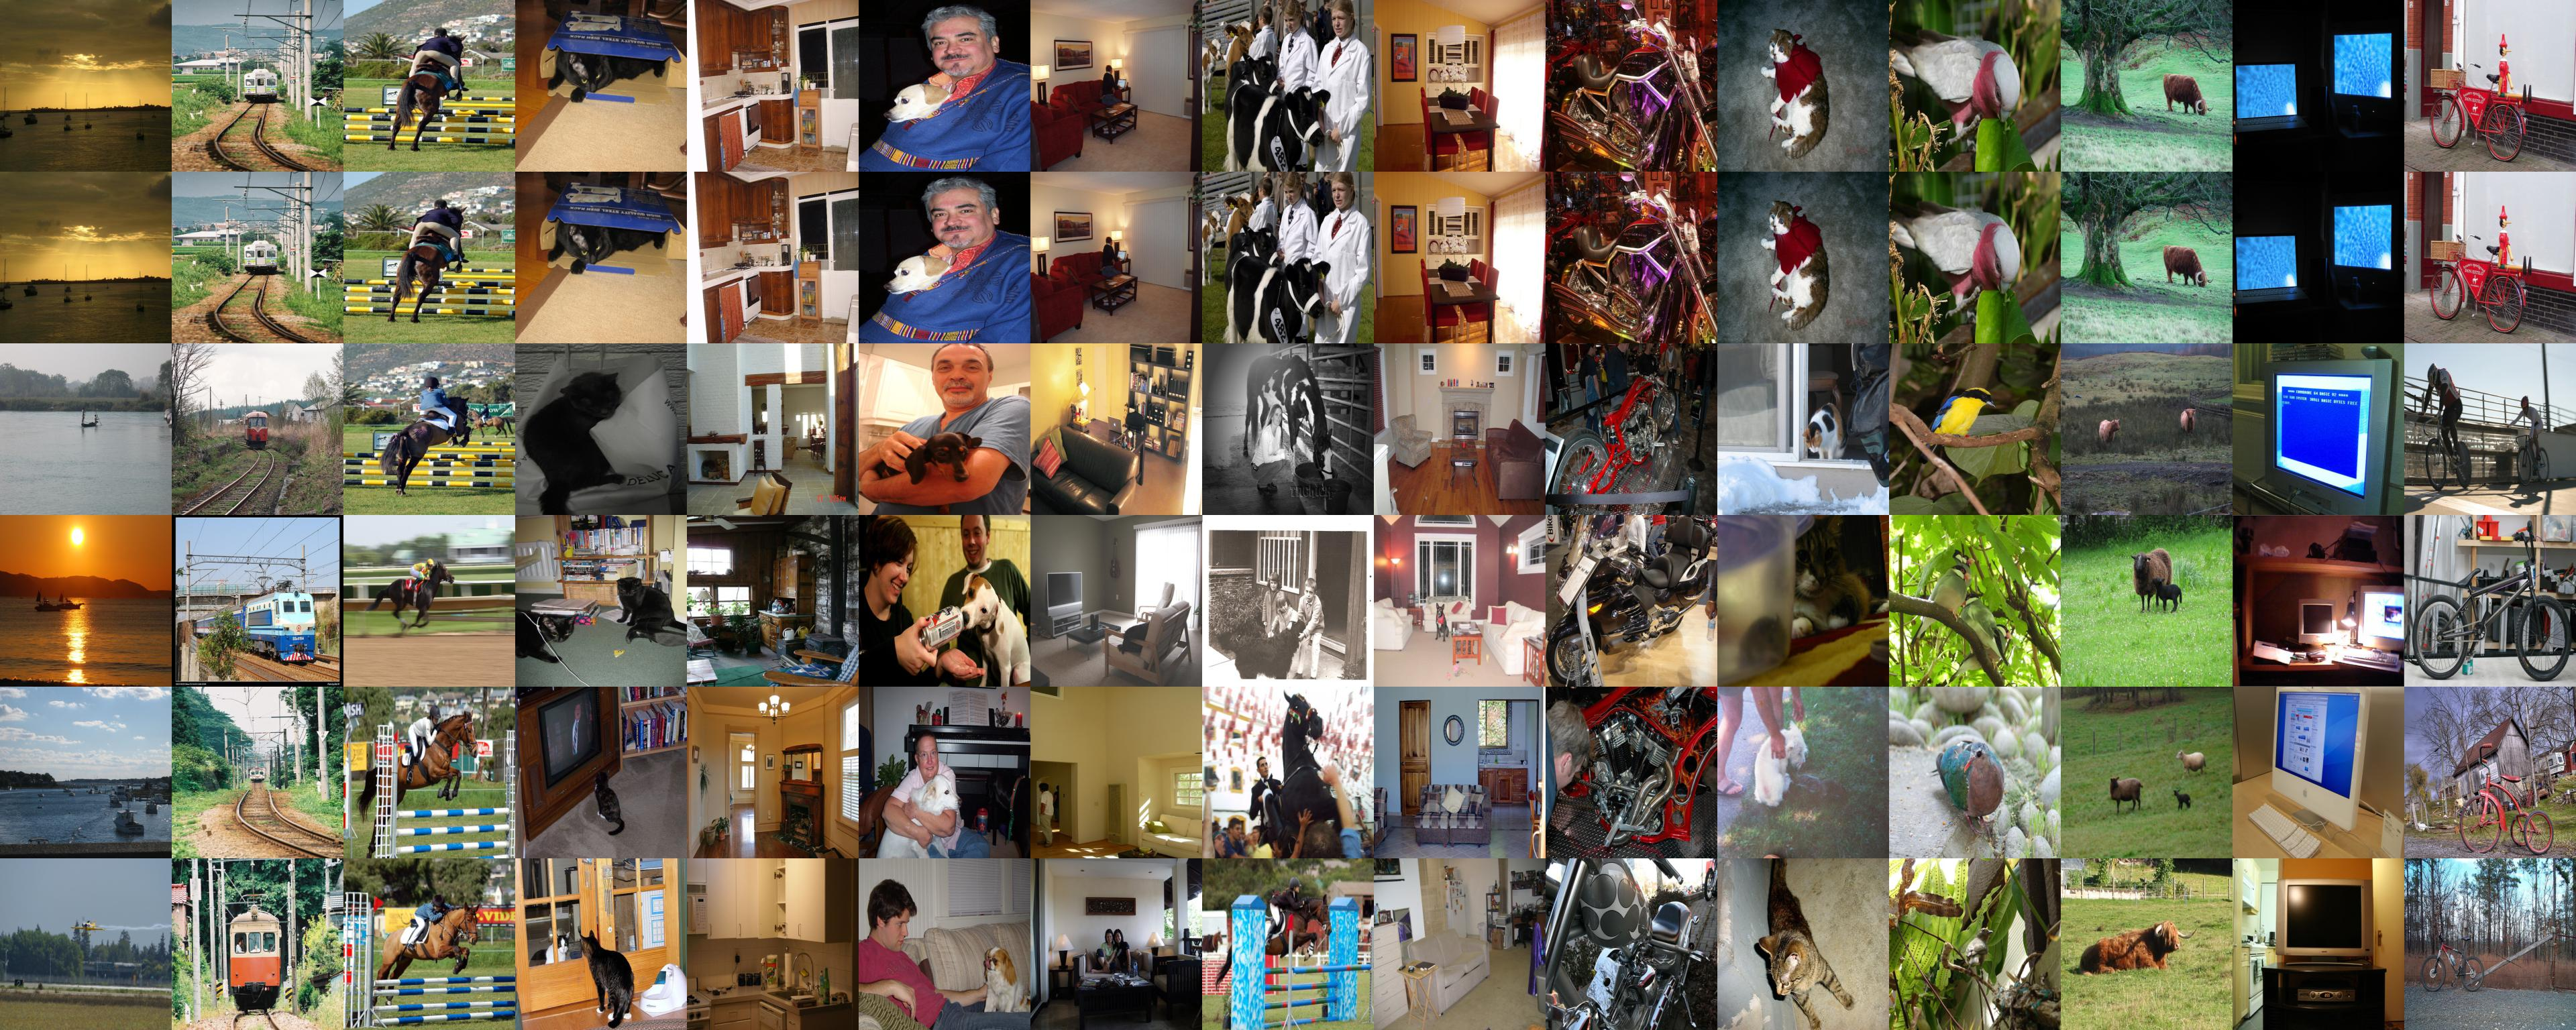
\includegraphics[width=7in]{task5_kNN_vgg16_fc7.jpg}}
  \caption{Task5: 5 Nearest Neighbours by pool5(a) and fc7(b) features of VGG16. The first line is the test images and lines below are their neighbours.}
  %\label{fig:subfig} 
\label{fig:short}
\end{figure*}

\textbf{tSNE visualization of intermediate features}\\

I randomly selected 1000 images from the test dataset and extracted fc7 features by AlexNet and VGG16 with pretrained model respectively. As the number of features of fc7 is too many, I first used PCA to get small dimensions of principal components. I tried 50, 200 and 400 as the number of components, but it turned out it's kind of invariant. Then, I fed the extracted features of PCA to the tSNE to project them into 2D plane and draw the image below.

As the AlexNet is not well-trained for PASCAL dataset, thus I can hardly find clustering phenomenon in the image. For VGG16, we can clearly see that the images of same kind clustered together. We can see that some classes like bicycle, car and aeroplane clustered very well. Some classes like cat and dog, which are similar to each other, locate very near each other in the figure. Classes like person locate among several clusters which may because the people always appear with other objects.\\ 

\begin{figure*}[!h]
  \centering
  \subfigure[]{
    \label{fig:subfig:a}
    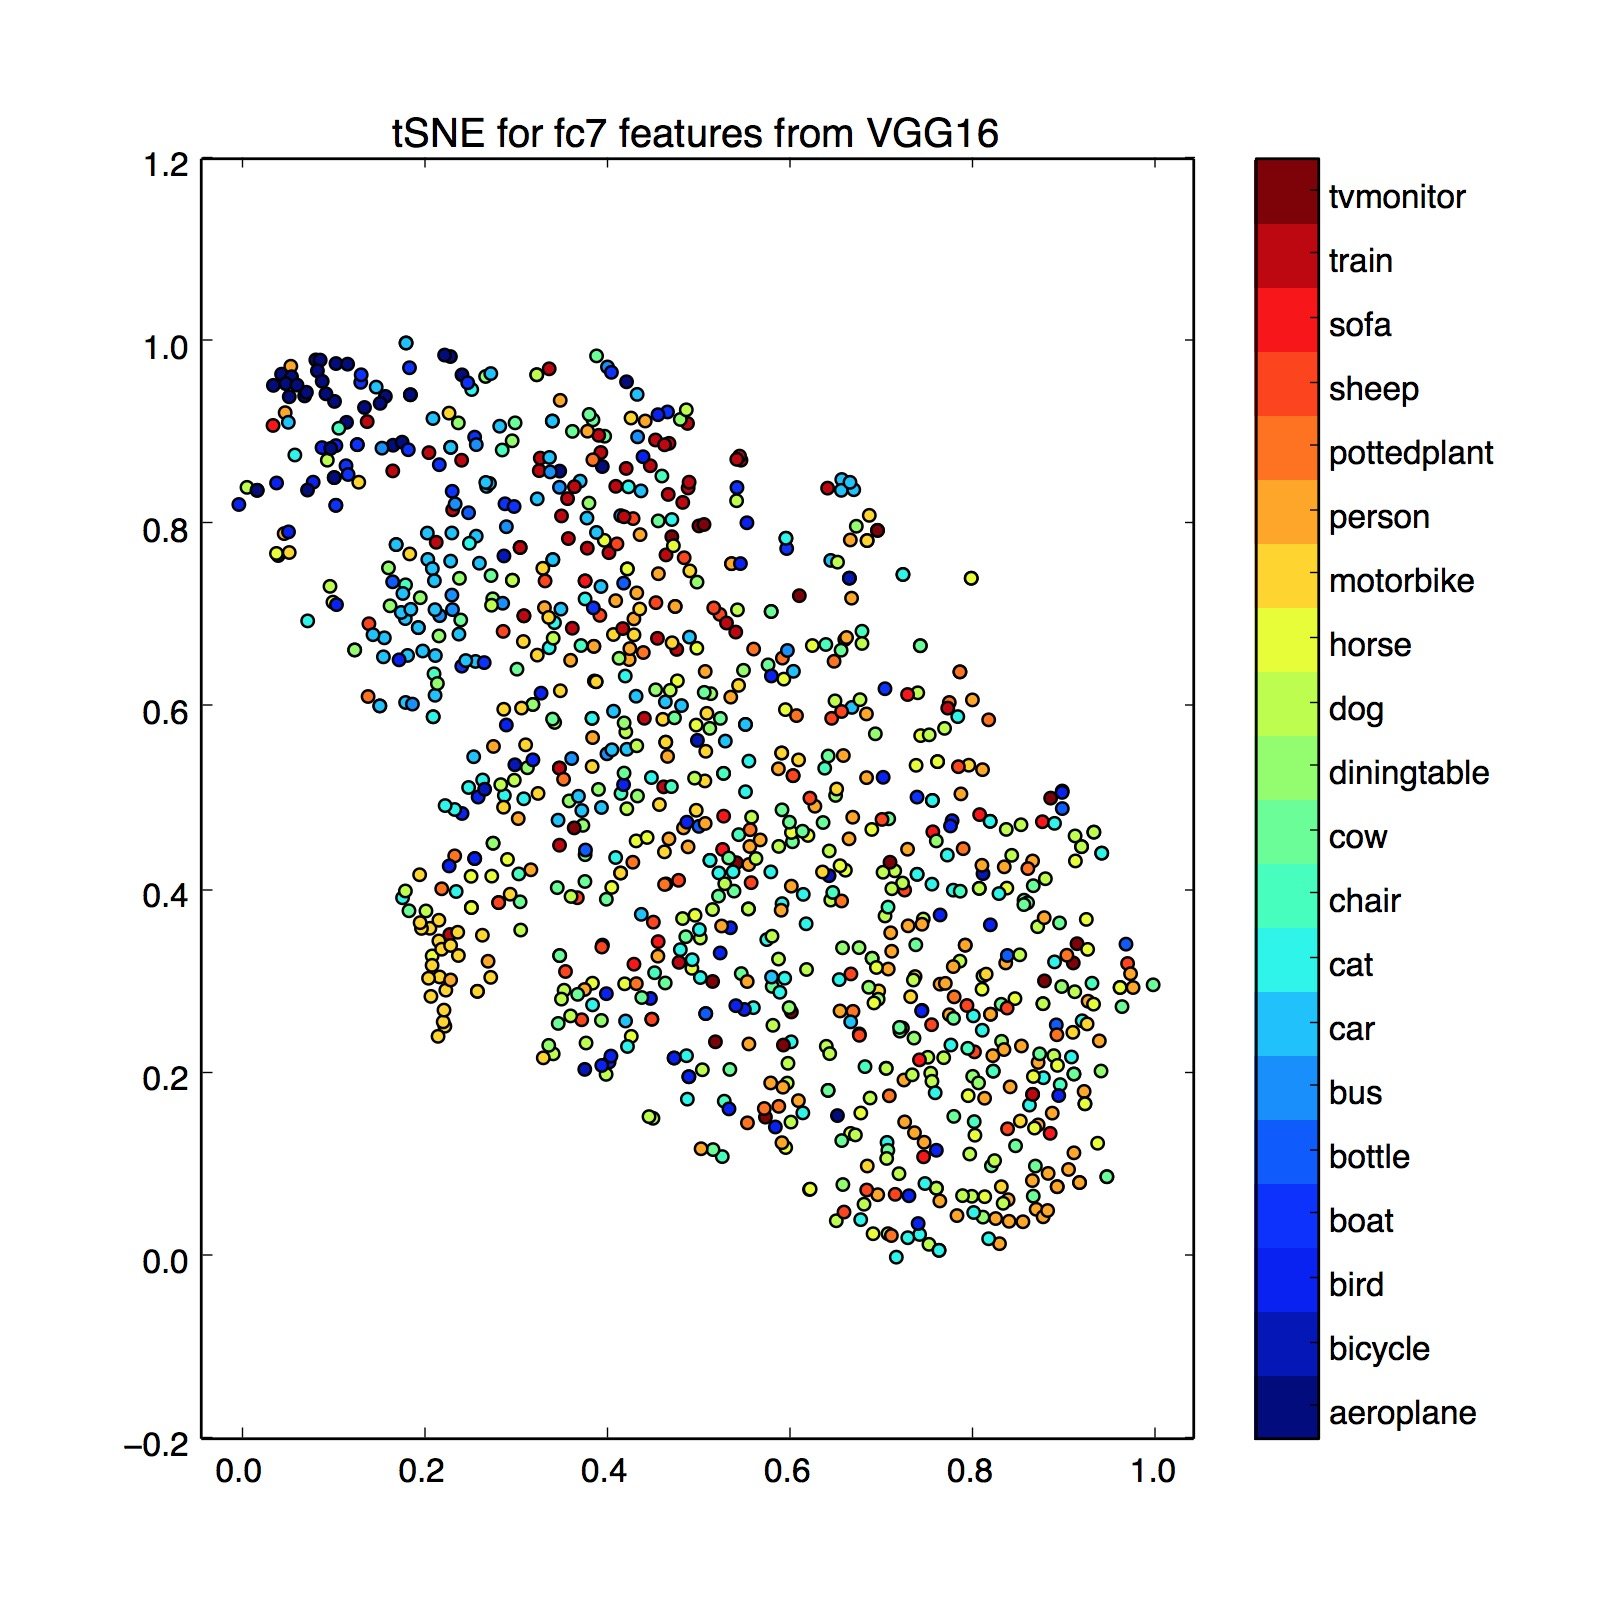
\includegraphics[width=4.5in]{task5_tSNE_alexnet_fc7_50.jpg}}
  %\hspace{0.01in}
  \subfigure[]{
    \label{fig:subfig:b} 
    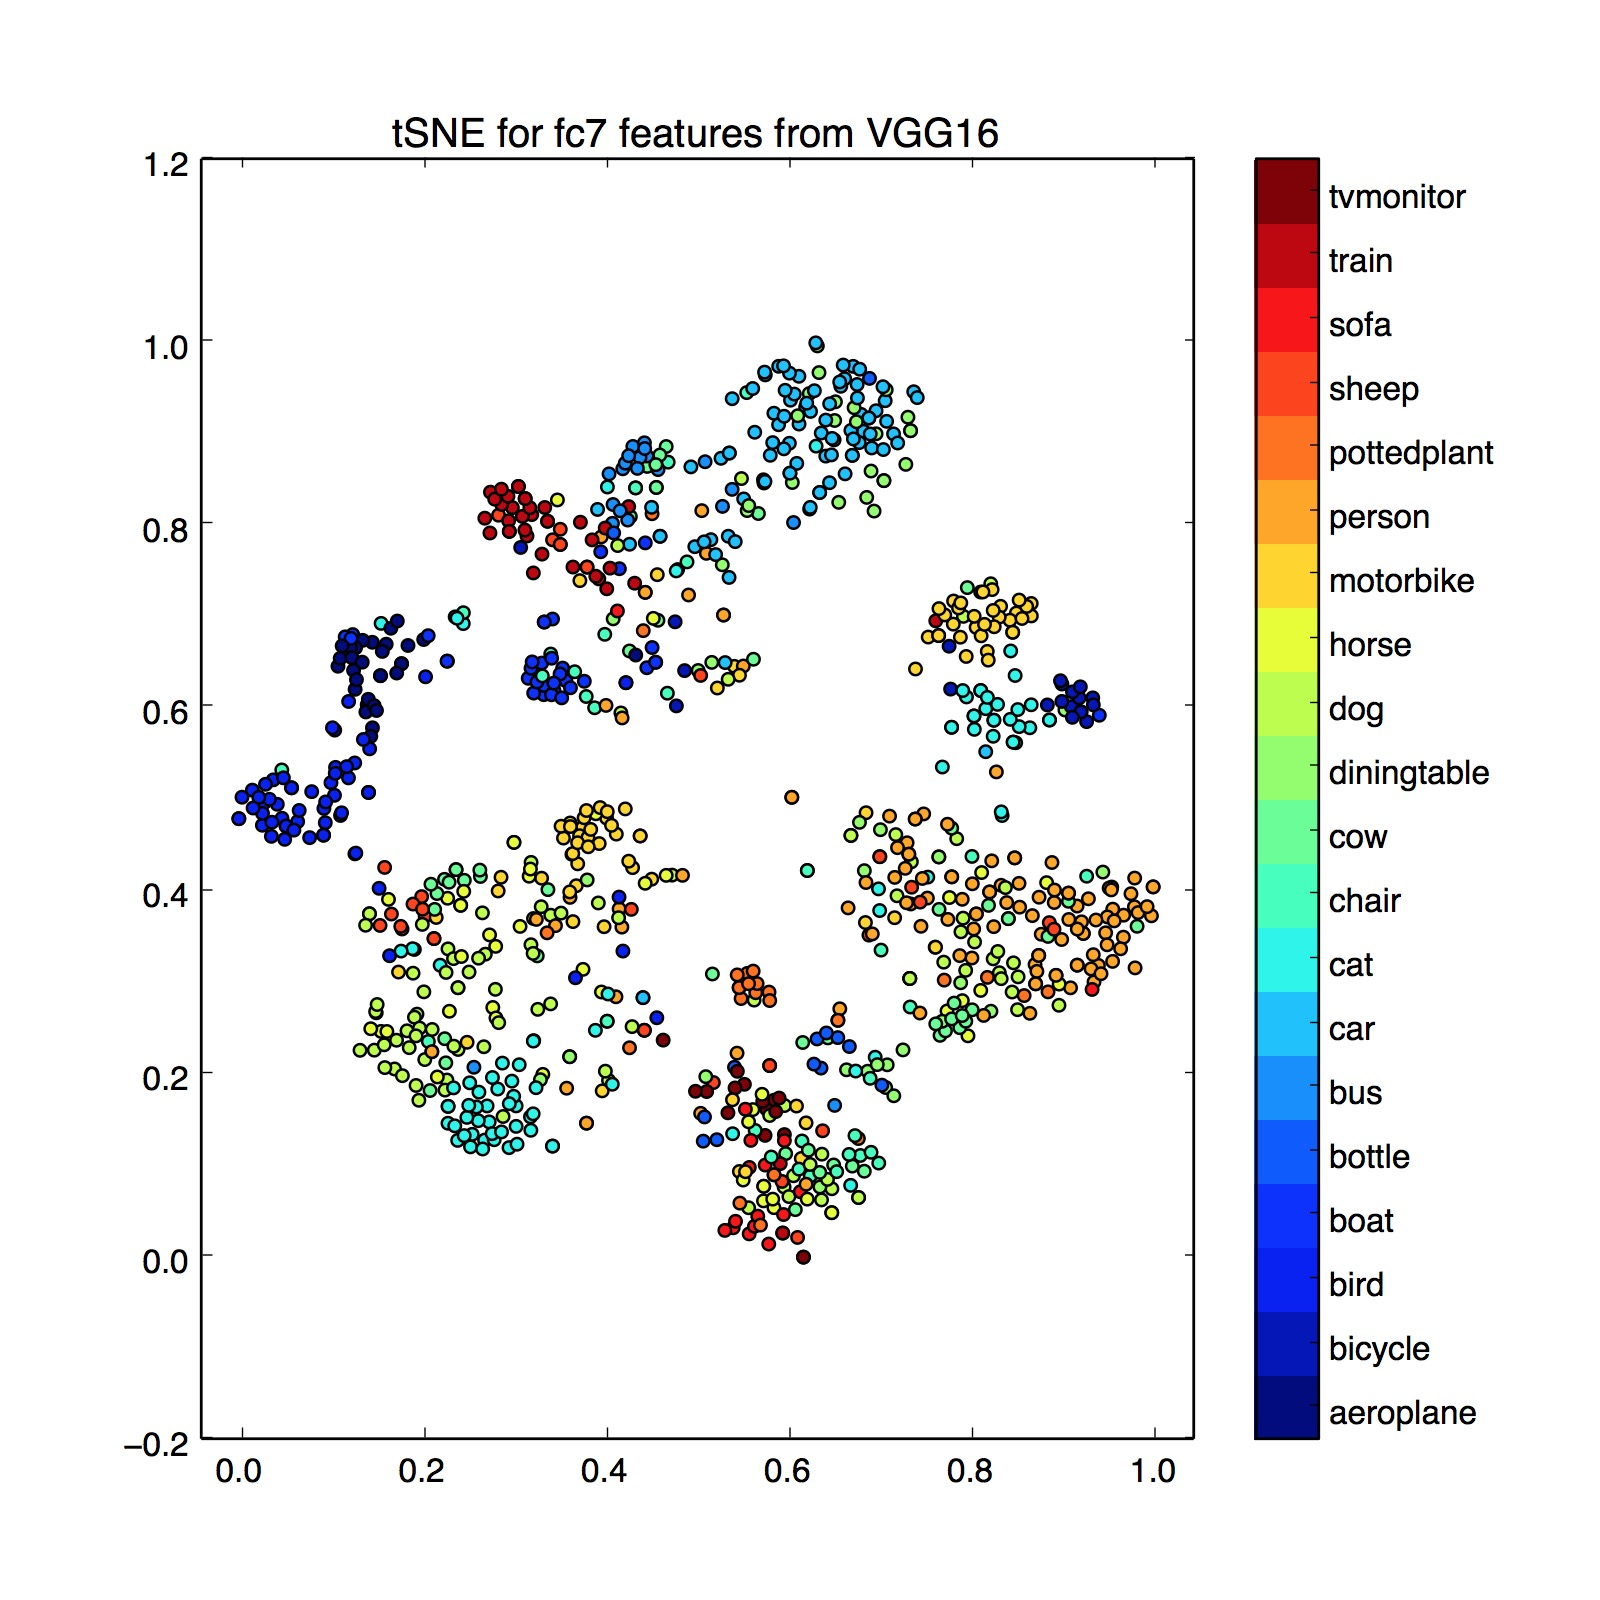
\includegraphics[width=4.5in]{task5_tSNE_vgg16_fc7_50.jpg}}
  \caption{Task5: tSNE results by fc7 in AlexNet(a) and VGG16(b). The component number of PCA is 50.}
  %\label{fig:subfig} 
\label{fig:short}
\end{figure*}

\textbf{Are some classes harder?}\\

As we can see from the table, the classes that achieve highest score are person and train, while the classes have lowest score are bottle and pottedplant. From random selected we can found that the images that contain person are much more than other classes, which may be the reason of achieving highest score. For train, its shape is rigid and normally takes large part of the image, which are easier for the network to learn. For the two classes with bad performance, the number of image that have these two is not much. Meanwhile, these two objects are normally very small and appear with other more dominant objects, thus the features are not fully extracted by the network.\\
Comparing to AlexNet, the accuracy of dog, cat and bird are largely improved, which may because there are many animal images in the ImageNet, thus the pretrained model can get better performance on these classes.\\



\begin{table}
\begin{center}
\begin{tabular}{c|c c c c c c c }
\hline
class & aeroplane & bicycle & bird & boat & bottle & bus & car \\
\hline
AlexNet & 0.61 & 0.34 & 0.23 & 0.33 & 0.13 & 0.20 & 0.55\\
VGG16 & 0.89 & 0.91 & 0.92 & 0.83 & 0.44 & 0.78 & 0.92\\
\hline
\hline
class & cat & chair & cow & diningtable & dog & horse & motorbike \\
\hline
AlexNet & 0.29 & 0.31 & 0.16 & 0.27 & 0.23 & 0.61 & 0.38\\
VGG16 & 0.91 & 0.62 & 0.63 & 0.72 & 0.88 & 0.88 & 0.89\\
\hline
\hline
class & person & pottedplant & sheep & sofa & train & tvmonitor &   \\
\hline
AlexNet & 0.74 & 0.15 & 0.28 & 0.26 & 0.37 & 0.24 &  \\
VGG16 & 0.98 & 0.52 & 0.72 & 0.64 & 0.96 & 0.68 &  \\
\end{tabular}
\end{center}
\caption{Per-class performance of AlexNet and VGG16 with pretrained model}
\end{table}

\item \textbf{Task 6 (Optional)}\\

The main idea of this mixup technique is do some linear interpolation of both features and labels to augment the training dataset. According to the paper, this method can increase the accuracy of classification and GAN training. But what I achieved is the opposite.\\
For AlexNet. I only achieved 26\% on overall mAP instead of the previous 33\%. For pretrained VGG16, I achieved 76\% instead of the previous 83\%. \\

\begin{figure*}[!h]
  \centering
  \subfigure[]{
    \label{fig:subfig:a}
    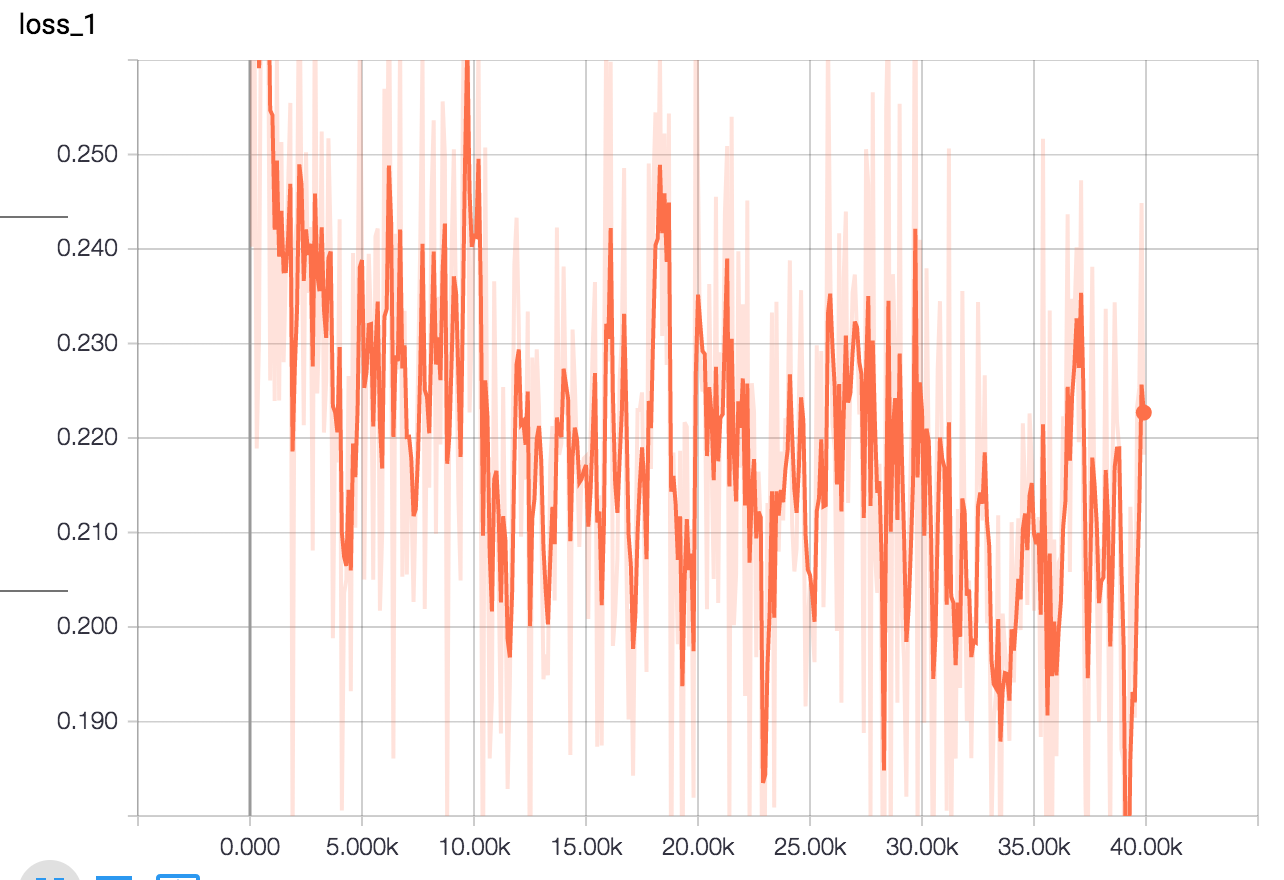
\includegraphics[width=3in]{task6_mixup_alexnet_loss.png}}
  %\hspace{0.01in}
  \subfigure[]{
    \label{fig:subfig:b} 
    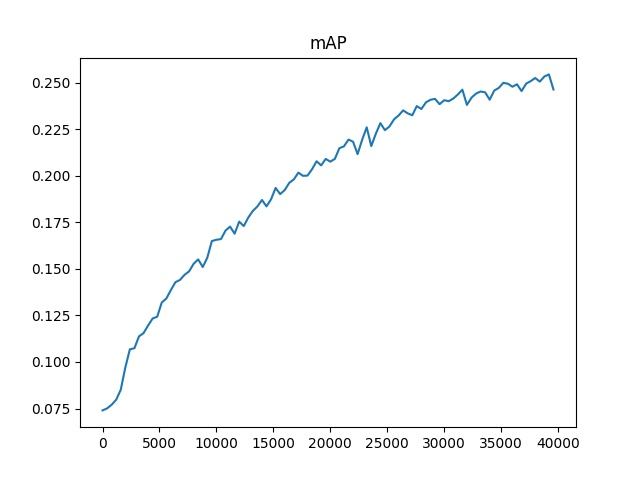
\includegraphics[width=3in]{task6_mAP_plot_alexnet.jpg}}
  \caption{Task6: Training and test curves of Mixup on AlexNet}
  %\label{fig:subfig} 
\label{fig:short}
\end{figure*}

\begin{figure}[!h]
  \centering
    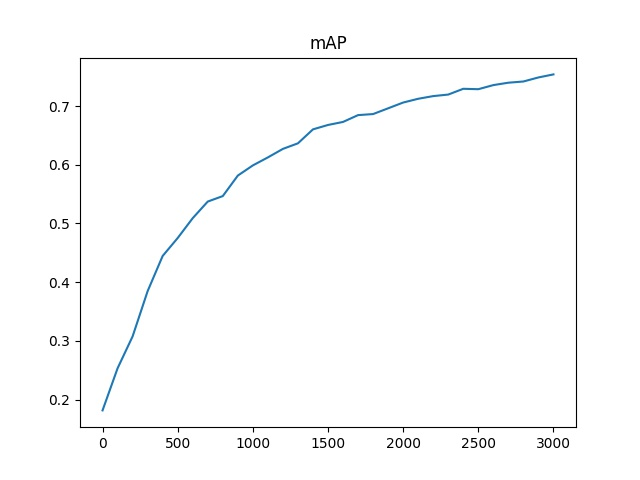
\includegraphics[width=3in]{task6_mAP_plot_vgg16_mixup.jpg}
  \caption{Task6: mAP curve of Mixup on pretrained VGG16}
\label{fig:short}
\end{figure}

\end{outline}
\end{document}